\documentclass[12pt,a4paper]{report}

\usepackage{szakd_report_win}
%\usepackage{szakd_report}
\usepackage{mathtools,xparse}

\DeclarePairedDelimiter{\abs}{\lvert}{\rvert}
\DeclarePairedDelimiter{\norm}{\lVert}{\rVert}

\newcommand{\TODO}{\colorbox{yellow}{\textbf{TODO}}}

\begin{document}
\pagestyle{empty} %a c�mlapon ne legyen semmi=empty, azaz nincs fejl�c �s l�bl�c

%A f�iskola logoja
{\large
\begin{center}
\vglue 1truecm
\textbf{\huge\textsc{Szakdolgozat}}\\
\vglue 1truecm

\epsfig{file=cimlap/ME_logo.eps, width=4.8truecm, height=4truecm}\\
\textbf{\textsc{Miskolci Egyetem}}
\end{center}}

\vglue 1.5truecm %f�gg�leges helykihagy�s

%A szakdolgozat c�me, ak�r t�bb sorban is
{\LARGE
\begin{center}
	Szakdoga címe
\end{center}}

\vspace*{2.5truecm}
%A hallgat� neve, �vfolyam, szak(ok), a konzulens(ek) neve
{\large
\begin{center}
\begin{tabular}{c}
\textbf{Készítette:}\\
Ferencsik Dorina Kinga\\
Évfolyam. szak-szak
\end{tabular}
\end{center}
\begin{center}
\begin{tabular}{c}
\textbf{Témavezető:}\\
Egyik konzulens neve\\
Másik konzulens neve\ldots
\end{tabular}
\end{center}}
\vfill
%Keltez�s: Hely �s �v
{\large
\begin{center}
\textbf{\textsc{Miskolc, 2019}}
\end{center}}

\newpage


\pagestyle{myheadings}

%Feladatkiiras
\begin{flushleft}
\textsc{\bfseries Miskolci Egyetem}\\
Gépészmérnöki és Informatikai Kar\\
Alkalmazott Matematika Tanszék \hspace*{4cm}\hfil \textbf{Szám:}
\end{flushleft}
\vskip 0.5cm
\begin{center}
\large\textsc{\bfseries Szakdolgozat Feladat}
\end{center}
\vskip 0.5cm

Ferencsik Dorina Kinga (YXI8DJ) 
programtervező informatikus 
jelölt részére
\newline

\noindent\textbf{A szakdolgozat tárgyköre:} numerikus eljárások tesztelése\newline

\noindent\textbf{A szakdolgozat címe:}\newline

\noindent\textbf{A feladat részletezése:}

\noindent Nemlineáris egyenletrendszer megoldására szolgáló ABS-módszerek áttekintő jellegű ismertetése.

\vfill

\noindent\textbf{Témavezető(k):} Dr. (vagy nem doktor) Valamilyen Valaki beosztás (pl. egyetemi adjunktus)\newline

\noindent\textbf{Konzulens(ek):} (akkor kötelező, ha a témavezető nem valamelyik matematikai tanszékről való; de persze lehet egyébként is)\newline

\noindent\textbf{A feladat kiadásának ideje:}\newline

%\noindent\textbf{A feladat bead�s�nak hat�rideje:}

\vskip 2cm

\hbox to \hsize{\hfil{\hbox to 6cm {\dotfill}\hbox to 1cm{}}}

\hbox to \hsize{\hfil\hbox to 3cm {szakfelelős}\hbox to 2cm{}}

\newpage

\vspace*{1cm}  
\begin{center}
\large\textsc{\bfseries Eredetiségi Nyilatkozat}
\end{center}
\vspace*{2cm}  

Alulírott \hbox to 7cm{\dotfill}; Neptun-kód: \hbox to 3.5cm{\dotfill} a Miskolci Egyetem Gépészmérnöki és Informatikai Karának végzős \hbox to 3.5cm{\dotfill} szakos hallgatója ezennel büntetőjogi és fegyelmi felelősségem tudatában nyilatkozom és aláírásommal igazolom, hogy \hbox to 9.5cm{\dotfill}
című szakdolgozatom/diplomatervem saját, önálló munkám; az abban hivatkozott szakirodalom
felhasználása a forráskezelés szabályai szerint történt\\

Tudomásul veszem, hogy szakdolgozat esetén plágiumnak számít:
\begin{itemize}
\item szó szerinti idézet közlése idézőjel és hivatkozás megjelölése nélkül;
\item tartalmi idézet hivatkozás megjelölése nélkül;
\item más publikált gondolatainak saját gondolatként való feltüntetése.
\end{itemize}

Alulírott kijelentem, hogy a plágium fogalmát megismertem, és tudomásul veszem, hogy
plágium esetén szakdolgozatom visszautasításra kerül.

\vspace*{3cm}

\noindent Miskolc, \hbox to 2cm{\dotfill} .év \hbox to 2cm{\dotfill} .hó \hbox to 2cm{\dotfill} .nap

\vspace*{3cm}

\hspace*{8cm}\begin{tabular}{c}
\hbox to 6cm{\dotfill}\\
Hallgató
\end{tabular}



\newpage

\noindent 1.

\begin{tabular}{cl}
&szükséges (módosítás külön lapon) \\
A szakdolgozat feladat módosítása& \\
& nem szükséges\\
&\\
\hbox to 4cm{\dotfill}&\multicolumn{1}{c}{\hbox to 5cm{\dotfill}}\\
dátum& \multicolumn{1}{c}{témavezető(k)}
\end{tabular}
\vskip1.5mm

\noindent 2. A feladat kidolgozását ellenőriztem:

\vskip1.5mm

\begin{tabular}{l@{\hspace*{4cm}}l}
témavezető (dátum, aláírás):& konzulens (dátum, aláírás):\\
\dotfill&\dotfill\\
\dotfill&\dotfill\\
\dotfill&\dotfill
\end{tabular}

\vskip1.5mm

\noindent 3. A szakdolgozat beadható:

\vskip1.5mm

\begin{tabular}{@{\hspace*{1.3cm}}c@{\hspace*{2.1cm}}c}
\hbox to 4cm{\dotfill}&\multicolumn{1}{c}{\hbox to 5cm{\dotfill}}\\
dátum& \multicolumn{1}{c}{témavezető(k)}
\end{tabular}

\vskip1.5mm

\noindent 4.
\begin{tabular}[t]{@{}l@{\hspace*{1mm}}l@{\hspace*{1mm}}l@{}}
A szakdolgozat& \hbox to 3.5cm{\dotfill} &szövegoldalt\\
              & \hbox to 3.5cm{\dotfill} &program protokollt (listát, felhasználói leírást)\\
              &\hbox to 3.5cm{\dotfill}   &elektronikus adathordozót (részletezve)\\
              &\hbox to 3.5cm{\dotfill} & \\
              &\hbox to 3.5cm{\dotfill} &egyéb mellékletet (részletezve)\\
              &\hbox to 3.5cm{\dotfill} &\\
\end{tabular}
\newline tartalmaz.

\vskip1.5mm

\begin{tabular}{@{\hspace*{1.3cm}}c@{\hspace*{2.1cm}}c}
\hbox to 4cm{\dotfill}&\multicolumn{1}{c}{\hbox to 5cm{\dotfill}}\\
dátum& \multicolumn{1}{c}{témavezető(k)}
\end{tabular}

\noindent 5.

\begin{tabular}{ll}
&bocsátható\\
A szakdolgozat bírálatra& \\
& nem bocsátható\\
\end{tabular}

\vskip1.5mm

\noindent A bíráló neve: \hbox to 8cm{\dotfill}

\vskip4mm

\begin{tabular}{@{\hspace*{1.3cm}}c@{\hspace*{2.1cm}}c}
\hbox to 4cm{\dotfill}&\multicolumn{1}{c}{\hbox to 5cm{\dotfill}}\\
dátum& \multicolumn{1}{c}{szakfelelős}
\end{tabular}

\noindent 6.
\begin{tabular}[t]{@{}l@{\hspace*{1mm}}l@{\hspace*{1mm}}l@{}}
A szakdolgozat osztályzata& &\\
&a témavezető javaslata:& \hbox to 3cm{\dotfill}\\
&a bíráló javaslata:& \hbox to 3cm{\dotfill}\\
&a szakdolgozat végleges eredménye:& \hbox to 3cm{\dotfill}
\end{tabular}

\vspace*{4mm}

\noindent Miskolc, \hbox to 4.5cm{\dotfill} \hspace*{2.5cm}
\begin{tabular}[t]{cc}
\hbox to 6cm{\dotfill}\\
a Záróvizsga Bizottság Elnöke
\end{tabular}
%feladat ki�r�s

\tableofcontents %automatikus tartalomjegyz�k--v�ltoz�s eset�n k�tszer ford�tani

\newpage

\pagestyle{fancy} %az oldal st�lusa, ez adja az al�h�zott fejlecet

%Az első fejezet
\Chapter{Bevezetés}
\label{Chap:bevezetes}
%1-4 oldal

A gépi tanulás egy egyre szélesebb körben használt és alkalmazott informatikai ág, mely az egyszerű levélszemét szűréstől a képfelismerésen és hangfeldolgozáson át rengeteg területen fontos szerepet játszik. Célja mindig meglévő adatok elemzése, egyfajta tanulási folyamat, amely után a jövőben új adatokra valamilyen becslés készíthető. Ennek az ágazatnak az al-területei nagyon szétágazóak, rengeteg létező megvalósítással. Általánosságban a tanulási módszer és a cél szerint csoportosíthatóak:
\begin{itemize}
	\item felügyelt tanulás: az adatnak része az információ amelynek a becslése a cél. A felügyelt módszerek csoportjába tartozó algoritmusok a magyarázó jellemzőket tartalmazó $X$ adathalmaz alapján tanulják meg a függő $y$ változó értékeit, általában valamilyen közelítést alkalmazva. A gépi tanulási módszerek nagyobb része ide sorolható.
	\item felügyelet nélküli tanulás: ebben az esetben az adathalmaz nem tartalmazza a függő $y$ változót, nem tudni hogy mire kell becslést készíteni. Jellemzően ide tartoznak a különböző klaszterezési eljárások, ahol valamilyen szempontból hasonló adatpontok csoportokba rendezése a cél, anélkül hogy az adatok hovatartozásáról bármilyen információ ismert lenne. 
\end{itemize}

A különböző gépi tanulási módszerek terjedésével a sport világában is hamar megjelent az alkalmazásuk, azonban elsősorban a profi, versenyzői szférában ahol régebb óta általános a sportolói eredményekre vonatkozó adatok gyűjtése, valamint természetesen nagyobb a pénzügyi forgás mint a hobbi sportolók esetében. Szakdolgozatom célja ebből kifolyólag a mindennapi, hobbi sportolók eredményeinek feldolgozása gépi tanulási módszerekkel, hiszen ez egy olyan terület ahol még nem sok megoldás létezik, azonban egyre nagyobbak a felhasználói igények.

A konkrét megvalósításhoz kerékpáros teljesítmények felhasználása került kitűzésre, egyrészt saját érdeklődési kör miatt, másrészt a kerékpáros útvonalak egyszerű mérhetőségéből és az adatok sokszínűségéből kifolyólag. Az így kitűzött adathalmaz specifikusságából eredően az adatgyűjtési folyamat is a szakdolgozat részét képezi, ami magába foglalja egy erre a célra készített weboldal megtervezését és kialakítását.






%Először 2018. nyarán kezdtem el az adatbányászattal és gépi tanulással foglalkozni és ahogy mind többet értettem meg belőle inkább érdekelt a terület, a kihívásai. A lelkesedés kitartott így ősszel a témaválasztás határidejének közeledtével az lebegett a szemem előtt hogy a területhez szorosan kapcsolódó szakdolgozatot tudjak elkezdeni.
 
%Az irány megszabása után egy konkrét célt kellett találni, egy alkalmazási területtet ahol a gépi tanulás jól hasznosítható, olyan problémák, feladatok vannak amihez érdemes lehet gépi tanulás algoritmusokat használni. Hosszas mérlegelés után a különböző sportok közül a kerékpározásra esett a választás. Ennek több oka is volt. Elsősorban a kerékpározás népszerű, elterjedt mozgásforma, így esélyesnek tűnt hogy viszonylag nagy mennyiségű statisztikai adatot lehet róla gyűjteni, változatos sportolói körből. Továbbá mikor időm engedi én is kerékpározok és ezeket az utakat rögzítem, így néhány kiinduló adat már elérhető volt ami alapján el tudtam kezdeni a tervezést. Az utak nyomon követésére a Strava mobil és webes alkalmazás szolgált, ami részletesen tárolja az egyes útvonalak statisztikai adatait. Az elérhető adatokat elemezve behatároltam több feladatot mint pl.:
%\begin{itemize}
%	\item Egy adott útvonal jellemzőinek ismeretében a teljesítéshez szükséges várható időtartam meghatározása. Ez az időtartam két részre választható szét, megkülönböztetjük a mozgással töltött időt a teljes eltelt időtartamtól ami a mozgási időből és a járulékos időveszteségekből adódik mint a forgalmi lámpánál várakozás, pihenés, hosszabb utak esetén étkezés.
%	\item Már megtett utak csoportosítása, nehézségi fokozatok meghatározása.
%	\item A nehézségi szintek alapján edzéstervek készítése.
%\end{itemize}

%Azonban a sportteljesítmény becslése nehéz feladat, mivel egyénenként nagyon eltérő, valamint az út nyers adatain kívül az egyén pillanatnyi fizikai és szellemi állapota is nagyban befolyásolja a teljesítményét (álmosság, kimerültség, kedvtelenség stb.). Ezért el kell dönteni hogy egy általános modell megépítése a cél, ami esetleg életkor, nem, edzettségi szint szerint finomhangolható azonban kisebb pontossággal rendelkezik, vagy személyre szabott, pontos becsléseket kell elérni ahol viszont a gépi tanulás során nehézséget okozhat a kis méretű adathalmaz, hiszen kevesen rendelkeznek akár csak egy-két ezer rögzített úttal, míg a megfelelő pontossághoz az egyes algoritmusoknak ennél nagyságrendekkel több adatra van szüksége.
 
%Az elsődleges cél általános modellek építése, ahol egy feladat megoldásához különböző gépi tanulási algoritmusokat lehet alkalmazni, ezeket egyenként javítani, maximalizálni a pontosságukat. Utána pedig az algoritmusokat össze kell hasonlítani a teljesítményük, felhasznált módszertanaik alapján.




\Chapter{Téma elméleti kifejtése}
\label{Chap:tema}

\Section{Mobil alkalmazások}
Napjainkban rengeteg különböző kerékpáros alkalmazás érhető el amik más más területre fókuszálnak. A következő pontokban ezekre láthatunk néhány példát az egyszerű mérnöki alapú számítástól az útvonalak nyomon követésén keresztül a fejlett, összetett tervező rendszerekig. Látható hogy a felhasználók körében nagy népszerűségnek örvend a különböző alkalmazások közösségi funkciói ahol lehetőség van az ismerősök megtalálására, útvonalak megosztására.  

\SubSection{Bike calculator}
A "Bike Calculator" \cite{bikecalculator} weboldal és mobil alkalmazás biciklis becsléseket kínál a felhasználói számára, teljesen mérnöki szempontból. A modell figyelembe veszi a sebesség, erőkifejtés, szélellenállás, gravitáció és egyéb tényezők összefüggését azonban egy általános eredményt ad, nincs lehetőség a felhasználó egyéni teljesítményének figyelembe vételére. Ezzel együtt is egy érdekes megoldás ami rengeteg paramétere révén jól skálázható.

\SubSection{Strava}
A Strava \cite{strava} az egyik legelterjedtebb alkalmazás a sporttevékenységüket nyomon követni kívánók körében, széles funkcionalitással és hatalmas felhasználói bázissal. Lehetőséget nyújt többek között biciklizés, futás, úszás, hegymászás és rengeteg egyéb sportág eredményeinek rögzítésére és korlátozott szintű tervezésére. A tevékenység során rögzített adatokból alapvető statisztikákat készít a felhasználók számára, mint a sebesség és a tengerszint feletti magasság változása valamint a sportoló pulzusának mozgása. Népszerűsíti a Strava-t hogy lehetőséget kínál az ismerősök megtalálására és az útvonalak, tevékenységek megosztására valamint kommentek és "kudo"-k egyfajta elismerés, tetszés nyilvánítás adására. Érdekes funkciói közé tartozik a szegmensek, rövid útvonal szakaszok kezelése ahol a felhasználóknak lehetőségük van rövid távon versenyezni, előrébb kerülni a szegmenst teljesítők listáján valamint számon tartani a saját rekordjaikat. 

A Strava tervezője, jövővel kapcsolatban segítő funkciója egy útvonal tervezőben merül ki,ami segíti a felhasználókat a legnépszerűbb út megtalálásában A és B pont között, térképpel és részletes navigációs leírásokkal. Az útvonal kijelölésénél az alapvető adatokon kívül egy becslést is kapunk a várható időre nézve. A várható idő számolása a bejelentkezett felhasználó legutóbbi 4 heti teljesítménye alapján történik. Előrelépés hogy egyáltalán figyelembe veszi a felhasználó eddigi útvonalait azonban ennek a módszernek is vannak hiányosságai így csak egy közepes kiindulási alapot ad. Alapvető gond ezzel a becsléssel hogy az útvonalak rögzítésénél a felhasználó hiába állítja be az út típusát (verseny, edzés, ingázás stb.) a Strava számítás során ezeket nem veszi figyelembe, így könnyen előfordulhat hogy a felhasználó kiugróan pontatlan, akár használhatatlan eredményt kap. Például az előző hetekben a saját határait feszegetve versenyre készült, most viszont szeretne egy nyugodt családi biciklizésre elindulni - ekkor nyilván nem fog rekordokat dönteni és a Strava által számolt várható idő semmilyen tényleges információval nem fog szolgálni számára.


\SubSection{Endomondo}
Az Endomondo \cite{endomondo} webes és mobil alkalmazás sporttevékenység nyomon követését hivatott megkönnyíteni a felhasználói számára. Rengeteg különböző sportágat megkülönböztet, ezekről külön statisztikákat készít valamint egyéni célokat lehet ezekre vonatkozóan beállítani. Az egyes sportágakat GPS alapú jelkövetés segítségével lehet nyomon követni, illetve kézzel is létrehozhatóak új tevékenységek, továbbá lehetőség van különböző alkalmazásokból vagy fájlból importálni korábban teljesített útvonalakat. Az alkalmazás megvalósít közösségi funkciókat is, a felhasználóknak lehetőségük van megkeresni az ismerőseiket akikkel később megoszthatják legújabb sporttevékenységüket valamint versenghetnek egymással a közösen felállított célok eléréséért. Az Endomondo érdekes adaléka hogy mozgás közben audió visszajelzést biztosít a felhasználók számára az addigi teljesítményükről, így a felhasználók sportolás közben is pontos információval rendelkezhetnek anélkül hogy az alkalmazást futtató eszközüket kellene figyelniük.


\SubSection{Best Bike Split}
A Best Bike Split \cite{bestbikesplit} egy rendkívül összetett rendszer amely elsősorban versenyzők számára kínál széles funkcionalitást. Alapköve a versenytáv megtételének optimalizálása melynek keretei között személyre szabott, szakaszokra bontott tervet állít fel a felhasználó számára annak érdekében hogy a tervezett távot a lehető legjobb idő alatt teljesítse. Ez a terv alapul veszi a felhasználó biciklijének és felszerelésének a tulajdonságait (kerekek típusa, bicikli súlya, sisak kialakítása stb.) a preferált versenyzési módot (elhelyezkedés a verseny során, sík terep illetve emelkedő esetén) valamint már teljesített edzést, versenyeket és természetesen a teljesítendő verseny paramétereit. Prémium előfizetés használata során a kalkulációt befolyásolja a várható időjárás is. A rendszer használható tetszőleges útvonalakra azonban az átlag kerékpáros számára szükségtelenül bonyolult, összetett így elsősorban versenyzők számára hasznos.

\SubSection{Összefoglalás és célkitűzés}
Több tucatnyi hasonló alkalmazás létezik, webes felülettel illetve Android és iOS lefedéssel hiszen a kerékpározás fellendülőben van napjainkban, így egyre több alkalmazás készül a felhasználói igények kielégítésére mind versenyzők mind pedig hétköznapi felhasználók számára akiknek a biciklizés inkább közlekedési mint sport eszköz. Ezen alkalmazások felsorolása vagy részletezése nem célja ennek a szakdolgozatnak, azonban néhány példa alapján is könnyen meghatározhatóak általános csoportok amelyekbe a létező megoldások besorolhatóak.


\subsubsection{Útvonal rögzítés} 
A legalapvetőbb funkció amire különböző megoldások léteznek. A legegyszerűbb eszközök esetén például csak az aktuális sebesség és a távolság kerül megállapításra egy, a kerékre rögzíthető érzékelőnek a segítségével. Az érzékelő használatával számolni lehet hogy a kerék hányszor fordul körbe adott időablakon belül, ennek és a kerék méretének felhasználásával könnyen megállapítható a pillanatnyi sebesség illetve az útvonal kezdete óta megtett távolság. Azonban a növekvő igényekhez igazodva ma már lényegesen elterjedtebbek a GPS alapú mobil alkalmazások amik a pillanatnyi sebességen és távolságon kívül pontosan tudják rögzíteni az út egyéb paramétereit is mint pl.: kezdő és végpont koordinátái, mozgással töltött idő, megtett emelkedő, legalacsonyabb és legmagasabb pont, átlag sebesség, maximum sebesség. Ezek a jellemzők lényegesen pontosabb leírást adnak egy-egy útvonalról, tárolásukkal könnyen nyomon követhető a személyes fejlődés, kitűzhetőek heti, havi, éves célok. Az útvonal paramétereinek nyomon követése, struktúrája és tárolása megvalósításonként változó, azonban a cél mindig ugyanaz: minél több jellemző meghatározása a lehető legrészletesebb módon.

\subsubsection{Közösségi funkciók} 
A kerékpáros útvonalakat nyomon követő mobil alkalmazások elterjedésével egy új tendencia jelent meg; egyre többször figyelhető meg valamilyen jellegű közösségi funkció megvalósítása az alkalmazáson belül, amik nagy népszerűségnek örvendenek az alkalmazást használók körében. Ezen funkciók nagyban különbözhetnek, általánosságban lehetőség van az alkalmazást használó ismerősök megtalálására, megtett útvonalak megosztására illetve valamilyen formában tetszésnyilvánítás / elismerés adására. Ezeken kívül általában megjelenik valamilyen ösztönzés, lelkesítés ami segíthet a teljesítmény javításában, a kitűzött célok elérésében. A Strava esetében ez a szegmensek formájában jelenik meg, amik lényegében rövid, maximum néhány száz méteres útvonalak, általában valamilyen szempontból nehezebb szakaszok (pl.: emelkedő). Ezen szegmensek teljesítésével a felhasználó automatikusan felkerül több rangsorra is (globális, adott évre vonatkozó, nem és korcsoport alapján lebontott) ahol lehetősége van ismerősökkel és ismeretlenekkel vetélkedni ezzel felébresztve a versenyszellemet. 

\subsubsection{Tervezés, becslés} 
A kerékpáros alkalmazások fejlődésének következő lépcsőfoka az útvonalak tervezése és a teljesítmény becslése. Útvonalak tervezésére kevésbé kerékpár specifikus alkalmazások is lehetőség adnak mint például a Google Térkép de sok, kifejezetten kerékpárosoknak készült alkalmazásban is léteznek megvalósítások. A tervezés különböző szempontok alapján történhet: egyik fontos szempont a távolság (ez a legfontosabb amennyiben a cél az út minél gyorsabb megtétele A és B pont között), egy másik pedig a népszerűség szóval foglalható össze. Az utóbbi főleg akkor fontos ha a kerékpározásra nem közlekedés szerűen tekintünk hanem inkább mint sport, kikapcsolódás hiszen ilyenkor előrébb kerül a jogos felhasználói igény az olyan útvonalakra ahol szép környezetben, lehetőség szerint autós és gyalogos forgalomtól zavartalanul lehet kerékpározni. Az útvonalak tervezéséhez szorosan kapcsolódik a teljesítmény, a várható idő meghatározása ami koránt sem egyszerű feladat. Ennek legalapvetőbb megoldása a Bike calculator által is megvalósított mérnöki, fizikai modell, ahol a teljesítmény tisztán a felszerelés és a megtenni kívánt út paraméterei alapján kerül kiszámításra


\subsubsection{Tervezés, becslés - egyéni teljesítmény alapján} 
Az útvonal tervezés és a várható teljesítmény becslésének továbbfejlesztésének, pontosításának alapjául az eddig megtett útvonalak és az elért eredmények szolgálhatnának, ez azonban egy olyan terület ahol még nem sok megoldás született. Ide sorolható a Strava által fejlesztett útvonal tervező, ahol a várható idő becsléséhez alapul veszi a bejelentkezett felhasználó elmúlt 4 heti teljesítményét, és míg ez egy jó kezdeményezés a valóságban nem mindig szolgál pontosabb információval mint egy egyszerű, fizikai összefüggéseken alapuló általános modell. Megnehezíti a pontos becslések készítését hogy egy adott felhasználó sokszor kevés adattal rendelkezik amelyek nem elég változatosak egy új útvonal esetén várható teljesítmény megbecsléséhez.\\[12pt]

\noindent
A fenti csoportok összefoglalása a vizsgált alkalmazásokra:
\begin{table}[!h]
	\resizebox{\textwidth}{!}{%
	\begin{tabular}{c|c|c|c|c|}
		\cline{2-5}
		\multicolumn{1}{l|}{} & 
		\multicolumn{1}{l|}{\textbf{Bike calculator}} & 
		\multicolumn{1}{l|}{\textbf{Strava}} & 
		\multicolumn{1}{l|}{\textbf{Endomondo}} & 
		\multicolumn{1}{l|}{\textbf{Best Bike Split}} \\ \hline
		
		\multicolumn{1}{|c|}{
			\begin{tabular}
				[c]{@{}c@{}}Útvonal \\ rögzítés
		\end{tabular}} & 
		{\color[HTML]{FE0000} $\boldsymbol{\times}$} & {\color[HTML]{009901} \textbf{\checkmark}} & {\color[HTML]{009901} \textbf{\checkmark}} & {\color[HTML]{009901} \textbf{\checkmark}}             \\ \hline
		\multicolumn{1}{|l|}{
			\begin{tabular}
				[c]{@{}l@{}}Közösségi \\ funkciók
		\end{tabular}} &
		{\color[HTML]{FE0000} \textbf{$\boldsymbol{\times}$}} & {\color[HTML]{009901} \textbf{\checkmark}} & {\color[HTML]{009901} \textbf{\checkmark}} & {\color[HTML]{FE0000} $\boldsymbol{\times}$}         \\ \hline
		
		\multicolumn{1}{|c|}{
			\begin{tabular}
				[c]{@{}c@{}}Tervezés\\ (általános)
		\end{tabular}} & 
		{\color[HTML]{009901} \textbf{\checkmark}} & {\color[HTML]{009901} \textbf{\checkmark}} & {\color[HTML]{009901} \textbf{\checkmark}} & {\color[HTML]{009901} \textbf{\checkmark}}     \\ \hline
		
		\multicolumn{1}{|c|}{
			\begin{tabular}
				[c]{@{}c@{}}Tervezés\\ (egyéni)
		\end{tabular}}   &
		{\color[HTML]{FE0000} $\boldsymbol{\times}$} & {\color[HTML]{009901} \textbf{\checkmark}} & {\color[HTML]{FE0000} $\boldsymbol{\times}$} & {\color[HTML]{009901} \textbf{\checkmark}}             \\ \hline
	\end{tabular}
	}
\end{table}


\subsubsection{Célkitűzés}
Ezen 4 fő csoport közül az első három által meghatározott problémákra, igényekre mára már rengeteg, változatos módon megvalósított megoldás létezik, így ezeknek a tárgyalásától a továbbiakban eltekintünk. Azonban az utolsó probléma, a felhasználó egyéni teljesítményének figyelembe vétele egy nyitott terület, ahova nem sokan merészkedtek még, így a szakdolgozat során összehasonlításra kerülő gépi tanulási algoritmusok célja sportolói teljesítmény becslése. A teljesítményt természetesen nagy mértékben befolyásolja a kerékpáros felszerelések minősége és állapota, az útvonal terep és időjárás viszonyai azonban az egyén általános és pillanatnyi fizikai és szellemi állapota (kimerültség, kedvtelenség stb.) nem elhanyagolható tényező. Az átlagos értelemben vett teljesítmény több részre bontható le a kerékpározás kapcsán, melyek a szakdolgozat során külön kerülnek megválaszolásra.


%%%%%%%%%%%%%%%%%%%%%%%%%%%%%%%%%%%%%%%%%%%%

\Section{Megválaszolandó kérdések}
A sportteljesítmény becslése nehéz feladat, mivel egyénenként nagyon eltérő lehet, valamint az út nyers adatain kívül (távolság, emelkedő, időjárás) a egyén pillanatnyi fizikai és szellemi állapota is nagyban befolyásolja (álmosság, kimerültség, kedvtelenség stb.). Ezért el kell dönteni hogy egy általános modell megépítése a cél, ami esetleg életkor, nem, edzettségi szint szerint finomhangolható azonban kisebb pontossággal rendelkezik, vagy személyre szabott, pontos becsléseket kell elérni ahol viszont a gépi tanulás során nehézséget okozhat a kis méretű adathalmaz, hiszen kevesen rendelkeznek akár csak néhány száz rögzített úttal, míg a megfelelő pontossághoz ehhez nagyságrendekkel több adatra van szüksége az egyes algoritmusoknak




\SubSection{Nehézségi osztályok meghatározása}
A Strava-ról gyűjtött utak sok adatot tartalmaznak azonban nincsenek kategorizálva, így cél az eddig megtett utakat nehézség alapján több osztályba sorolni, azonban ennek megvalósítása kérdéses. Mivel a helyes label-ek hiányoznak klaszterezési módszereket kell használni. Várhatóan az egyén adatai alapján és a összes összegyűjtött adat alapján készült osztályok különbözőek lesznek, hiszen más útvonalakat tettek meg, eltérő eredményekkel.

Egy általános modell elkészítése az elsődleges feladat, mivel az adatok sokszínűsége és mennyisége miatt jobb kiindulópontot jelent. Amennyiben egy adott felhasználó megfelelően sok és sokféle útvonal adattal rendelkezik akkor érdemes lehet egyéni, személyre szabott nehézségi csoportok kialakításával is foglalkozni.

%\SubSection{Nehézség meghatározása - új útvonalra}
%A már megtett útvonalak osztályozása után a következő lépés az új, megtenni kívánt útvonalak nehézségének meghatározása. Ez megvalósítható egyrészt a már betanított klaszterezési algoritmusok felhasználásával, másrészt a klaszterezés által meghatározott osztályok label-jeit felhasználva valamilyen osztályozással. 


%Időpont is érdekes lehet (reggeli / esti között van e különbség)
\SubSection{Időtartam becslés}

Az egyik legalapvetőbb feladat a várható idő meghatározása, hiszen ez az egyik legmeghatározóbb pontja a kerékpározásnak - mennyi időbe fog telni mire megtesz valaki adott távolságot? Ennek a kérdésnek a megválaszolására alapvetően a különböző regressziók alkalmasak, amik az út paraméterei alapján folytonos értéket adnak vissza. Azonban ez a pont kicsit bonyolultabb mint amilyennek tűnik, mivel alapvetően kétféle időtartamot különböztetünk meg: a mozgási és a tényleges időtartamot. Az első jelöli az összesen mozgással töltött időt, míg a második magába foglalja a különböző megállókat mint a pihenés, várakozás forgalmi lámpáknál, hosszabb utak esetén étkezéssel töltött időket stb.

% Ennek megoldására több lehetőség is kínálkozik.

%A legegyszerűbb megoldás olyan regresszió használata amely egy inputhoz több eredmény, output-ot is tud társítani. Erre kínál lehetőséget \myaref{ssec:mlpregressor} pontban részletezett MLPRegressor. Ennek használatával rögtön mindkét idő előáll, nem szükséges további lépéseket tenni.

%A második lehetőség több részből áll. 
A különböző időtartamok kiszámításához első lépésben tetszőleges regresszióval csak a mozgási időre készül becslés, mivel ez szorosabban összefügg  az olyan alapvető adatokkal mint a távolság. Második lépésként pedig egy újabb regressziós modellt kell használni, ami a mozgási idő és egyéb paraméterek segítségével képes a teljes várható időre becslést készíteni.


\SubSection{Edzésterv}
%Nem útvonal meghatározása, hanem 

%1. mekkora távot mennyi idő alatt milyen emelkedővel stb. kellene megtennie hogy fejlődjön

%2. felhasználó által beadott út idejének becslése az alapján hogy normál / edzés szerű utat akar

%\TODO kifejtés

A felhasználók számára javasolt edzésterveknek több lehetséges megvalósítási módja is van. A legteljesebb kivitelezés a térképen jelölt konkrét útvonal, célul kitűzött teljesítési és részidőkkel, nehézségi szinttel. Azonban a szakdolgozat során egy lényegesen egyszerűbb, alapvető módszer megvalósítása a cél, aminek alapját a korábban meghatározott nehézségi csoportok fogják jelenteni. 

%%%%%%%%%%%%%%%%%%%%%%%%%%%%%%%%%%%%%%%%%%%

\Section{Gépi tanulás}
Rengeteg gépi tanulási módszer létezik amik jól használhatóak különböző modellek, becslések, osztályok készítésére. Ezek a módszerek ma már legtöbbször egy programozási nyelv adott könyvtárának, csomagjának segítségével egyszerűen használhatóak. Ennek megfelelően a Python nyelv scikit-learn \cite{scikitlearn} csomagja adta a gépi tanulási módszerek alapját a szakdolgozat elkészítése során.

Az egyes algoritmusok használatán túl fontos a megfelelő adatforrás megtalálása, valamint az adatkinyerési és feldolgozási folyamat leegyszerűsítése, átláthatóvá tétele. 

Ebben a fejezetben találhatóak meg a szakdolgozat során használt gépi tanulási módszertanok részletezése, valamint az adatgyűjtéshez létrehozott rendszer eszközeinek kifejtése.



\SubSection{Regresszió} \label{subsec:regression}
A regresszió egy felügyelt gépi tanulási módszer amely folytonos kimenetet generál. A tanuláshoz szükség van a bemeneti adathalmazra valamint a helyes kimeneti értékekre, amik elemzésével az algoritmus képes új bemeneti adatpárokra kimenetet generálni.

\subsubsection{Ridge}
A Ridge regresszió \cite{sklearn-ridge}\cite{ml-ridge} kitűnően alkalmas a Legkisebb négyzetek módszerének problémáinak való kiküszöbölésére. 
A módszer matematikailag:

$$ \min_{w} \norm{Xw-y}_2^2 + \alpha \norm{w}_2^2$$ 
ahol $\alpha \geq 0$ komplexitási paraméter. Ez a paraméter befolyásolja a csökkenés (\textit{shrinkage}) mértékét: minél nagyobb az $\alpha$ annál meredekebb a csökkenés. 

Érdemes használni mikor:
\begin{itemize}
	\item a magyarázó változók (jellemzők) száma meghaladja a vizsgálatok (adatsorok) számát egy adathalmazban
	\item a magyarázó változók (jellemzők) között korreláció figyelhető meg, tehát mikor az adathalmaz multikollineáris
\end{itemize}

Regularizáció: a Ridge regresszió L2-es típusú regularizációt valósít meg, azaz büntető kifejezésként (\textit{penalty term}) az $\alpha \norm{w}_2^2$ formula kerül felhasználásra.


Ridge és Legkisebb négyzetek módszere: a legkisebb négyzetek módszere nem különböztet meg "fontos" és "kevésbé fontos" jellemzőket, így magas jellemzőszám és kevés adatsor esetén túlilleszkedést eredményez, valamint nehezen kezel multikollineáris adathalmazt. A Ridge regresszió kiküszöböli ezeket a problémákat ugyanis pontosan elegendő torzítást (\textit{bias}) használ ahhoz, hogy a becslések ésszerűen megbízhatóak legyenek.



\subsubsection{Lasso}
A LASSO regresszió \cite{sklearn-lasso}\cite{ml-lasso} a \textit{Least Absolute Shrinkage and Selection Operator} angol kifejezés rövidítése. Ez egy lineáris modell amely ritka együtthatókat (\textit{sparse coefficients}) becsül. Hasznos lehet tömörített érzékelés (\textit{compressed sensing}) esetén mivel a kevesebb magyarázó változót tartalmazó megoldások felé tendál, így effektíve csökkentve az eredményt befolyásoló jellemzők számát. Matematikailag:

$$ \min_{w}\frac{1}{2n_{samples}} \norm{Xw-y}_2^2 + \alpha \norm{w}_1$$
ahol $\alpha \geq 0$ konstans együttható az L1 regularizációt befolyásoló, csökkenés mértékét jelző paraméter. 
\begin{itemize}
	\item $\alpha = 0$ esetén egyetlen jellemző sem kerül elvetésre, gyakorlatilag egy lineáris regresszió
	\item $\alpha$ növekedésével egyre több jellemző kerül elvetésre. Elméletileg $\alpha = \infty$ esetben minden jellemző elvetésre kerül
	\item $\alpha$ növekedésével nő az elfogultság (\textit{bias}). Magas bias esetén alulilleszkedés figyelhető meg.
	\item $\alpha$ csökkenésével nő a variancia (\textit{variance}). Magas variancia esetén túlilleszkedés figyelhető meg.
\end{itemize}

A Lasso regresszió tehát támogatja a minél egyszerűbb, ritka (\textit{sparse}) modelleket. Jól használható multikollineáris adathalmaz esetén illetve modell szelekció automatizálásához (pl.: magyarázó változók kiválasztása).



\subsubsection{Random Forest }
A Random Forest \cite{sklearn-randomforest}\cite{ml-randomforest} modell egy additív típusú modell amely a jellemzők közötti összefüggések feltárásához döntési fákat kombinál egy végső modellbe. Formálisabban:
$$ g(x) = f_0(x) + f_1(x) + f_2(x) + \dots$$
ahol a $g$ végleges modell az $f_i$ alapmodellek összessége. Minden $f_i$ egy döntési fa. A Random Forest érdekessége hogy az összes alapmodell egymástól függetlenül, a rendelkezésre álló adat különböző részhalmazait felhasználva kerül kialakításra.

A módszer előnye a lineáris modellekkel szemben hogy képes a nem-lineáris összefüggéseket is megtalálni a magyarázó és a függő változók között.



%\subsubsection{MLPRegressor} \label{ssec:mlpregressor}
%Multi-layer Perceptron Regression \cite{sklearn-mlpregressor}, azaz mesterséges neuronokból felépülő többrétegű struktúrán, más néven egy neurális hálón alapuló regressziót valósít meg. Ez egy felügyelt tanulási algoritmus, tehát inputként a feature-ok egy mátrixát ($X$) valamint a hozzájuk tartozó helyes label-eket ($y$) várja. Ezen értékek alapján backpropagation-t használva a módszer folytonos értékek készletével tér vissza. Az MLPRegressor továbbá több kimenetű regressziót is támogat, így egy mintához több output érték is rendelhető.


\SubSection{Klaszterezés} \label{ssec:klaszterezes}
A klaszterezés egy felügyelet nélküli gépi tanulási módszer, amelynek célja egy adathalmazt különálló csoportokra (klaszterekre) felbontani az adathalmazban fellelhető jellemzők alapján. A klaszterek kialakításakor a cél mindig valamilyen hasonlóság megtalálása az egyes adatpontok között, így az adott szempontból hasonló adatok fognak egy klasztert alkotni. Hasonlóság meghatározására rengeteg különböző módszer létezik, két legnagyobb csoportja körül az első a tömörséget, távolságot veszi alapul a második pedig a pontok kapcsolódását vizsgálja. Mindkét csoportban rengeteg különböző megvalósítás létezik.

\subsubsection{K-Means}
A K-Means \cite{sklearn-kmeans} eljárás az egyik legelterjedtebb, széles körben használt klaszterezési módszer, amely az adatpontokat távolságuk alapján csoportosítja. A módszer alapgondolata azonos szórású klaszterek kialakítása a tehetetlenség (\textit{inertia}) vagy másképp a klasztereken belüli négyzetösszegek minimalizálásával:
$$\sum_{i=0}^{n} \min_{\mu_j \in C} (|| x_i - \mu_j ||^2)$$,
ahol $n$ az $X$ adathalmaz darabszáma, $C$ a $c_j$ klasztereket tartalmazó halmaz és $\mu_j$ a $c_j$ klaszter középértéke, ami egyben a klaszter jellemzésére is szolgál. A $\mu_j$ pontot szokás középpontnak is nevezni, azonban ez az érték általában nem eleme az $X$ halmaznak. A K-Means algoritmus az $n$ mintát $K$ diszjunkt klaszterre osztja, ahol $K$ értékét előre definiálni kell.

A módszer jól teljesít nagy mennyiségű mintát tartalmazó adathalmazon azonban koránt sem tökéletes:
\begin{itemize}
	\item feltételezi hogy a klaszterek konvexek és izotrópok, ami természetesen nem mindig teljesül. Ebből kifolyólag rosszul teljesít hosszúkás vagy szabálytalan elrendezésű adaton
	\item a minimalizálásra kijelölt tehetetlenség nem normalizált mérőszám, annyit tudni róla hogy a kisebb értékek jobbak és nulla az optimális. Így az Euklideszi távolság használata miatt magas dimenziószámú adathalmaz esetén erősen ajánlott valamilyen dimenzió redukciós eljárás alkalmazása
\end{itemize}


\subsubsection{Mini-Batch K-Means }
%A MeanShift \cite{sklearn-meanshift}\TODO kifejtés
A Mini-Batch K-Means klaszterezési eljárás a K-Means egy variánsa, amely a számítási idő csökkentésének érdekében mini kötegeket (\textit{batch}) használ, ugyanakkor igyekszik optimalizálni ugyanazt a célfüggvényt. Ezek a mini kötegek az adathalmaz véletlenszerűen választott részhalmazai, amelyek az eljárás során egységként kezelve kerülnek hozzárendelésre a legközelebbi klaszter középponthoz. Más K-Means gyorsító eljárásokkal szemben a Mini-Batch előnye hogy általánosságban nagyon kicsit a eredmény romlása az alap K-Means-hez képest.

\subsubsection{Spectral}
A Spectral klaszterezési módszer \cite{sklearn-spectral} \cite{ml-spectral} a K-Means algoritmussal szemben nem a pontok távolsága alapján alakítja ki a klasztereket, hanem azok kapcsolatát veszi alapul: hiába esik közel egymáshoz két pont, amennyiben nem kapcsolódnak nem kerülnek egy klaszterbe. A módszer az adathalmazt egy alacsony dimenziójú térre vetíti le és itt alakít ki egy ún. affinitási mátrixot. Ez az affinitási mátrix tárolja hogy mely pontok kapcsolódnak egymáshoz: ehhez a pontok páronkénti távolságát vizsgálja. Két pont között akkor áll fent kapcsolat ha távolságuk kisebb mint valamilyen $\epsilon$ érték.

A Spectral és a K-Means algoritmusok különbözőségét a \myref{fig:spectralVSKmeans} ábra szemlélteti. Látható hogy míg a K-Means gyakorlatilag egy vonal mentén kettészeli az adathalmazt, nem törődve a spirális alakzattal, addig a Spectral klaszterezés a két spirál vonal alapján alakítja ki a két klasztert.
\begin{figure}
	\centering
	\includegraphics[width=0.9\textwidth,keepaspectratio]{kepek/spectral_vs_kmeans.png}
	\caption{K-Means és Spectral klaszterezés összehasonlítása \cite{ml-spectral-vs-kmeans-img}}
	\label{fig:spectralVSKmeans}
\end{figure}

%%%%%%%%%%%%%%%%%%%%%%%%%%%%%%%%%%%%%%%%%

\Section{A gépi tanulás alapköve - adatok}

A gépi tanulás módszerei önmagukban mit sem érnek, megfelelő méretű és minőségű adathalmazra van szükség amiből az algoritmusok tanulni tudnak. Azonban adatgyűjtés mindig érzékeny terület, sok időt, energiát felemészt és a kívánt eredmény ezek befektetésével sem mindig garantált. A szakdolgozathoz elsősorban biciklivel megtett utak statisztikai adataira van szükség, amihez a Strava mobil és webes alkalmazás ad kiindulási alapot. A fejlesztői munkát segíti a Strava saját API-ja, aminek segítségével egyszerűen megvalósítható a felhasználók autentikációja valamint a szükséges adatok elérése. 

\SubSection{Adatgyűjtés}
A Strava által gyűjtött és tárolt adatok elérésének alapját egy, a szakdolgozat keretein belül készített weboldal adja, amely a https://cycling-with-ml.firebaseapp.com címen érhető el. Ezen oldal felkeresésével a felhasználók tájékozódhatnak a szakdolgozatról, az adatgyűjtés fontosságáról valamint alapvető funkciókat használhatnak. Az oldalon lehetőség van új felhasználó létrehozására és már létező fiókokba való bejelentkezésre. Bejelentkezés után a felhasználó hozzákapcsolhatja a Strava fiókját a weblapon létrehozott fiókjához, ezzel lehetővé téve az útvonalai statisztikai adatainak olvasását. A weboldal az alábbi eszközök felhasználásával valósult meg:

\begin{figure}
	\centering
	\begin{subfigure}[b]{0.35\textwidth}
		\centering
		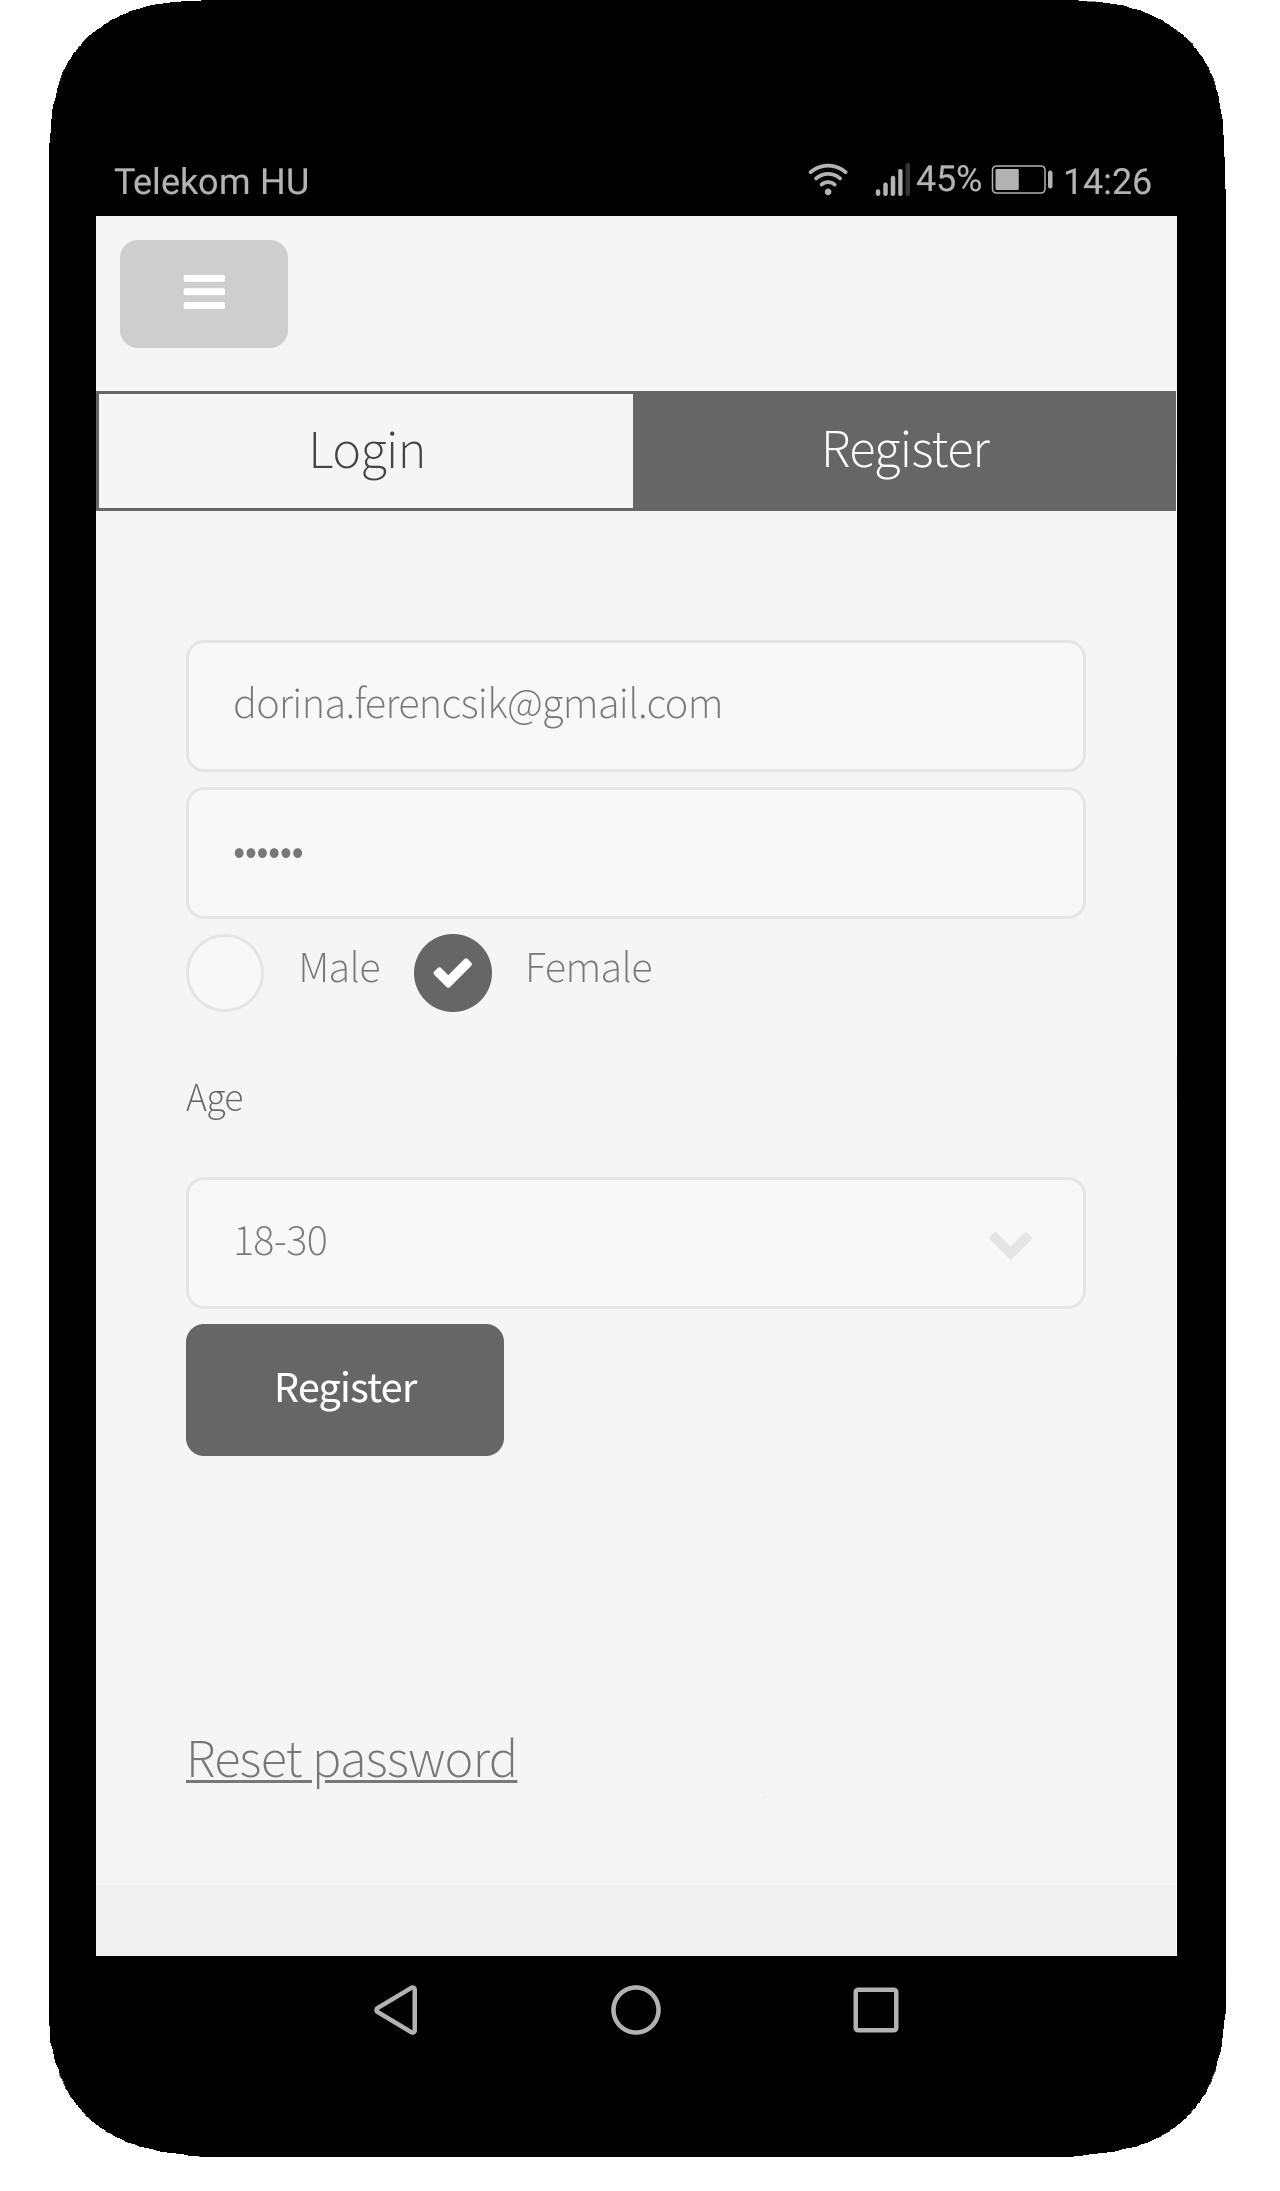
\includegraphics[ width=\textwidth,keepaspectratio]{kepek/website/websiteRegister.png}
		\caption{Regisztráció}
		\label{fig:websiteRegister}
	\end{subfigure}
	\begin{subfigure}[b]{0.35\textwidth}
		\centering
		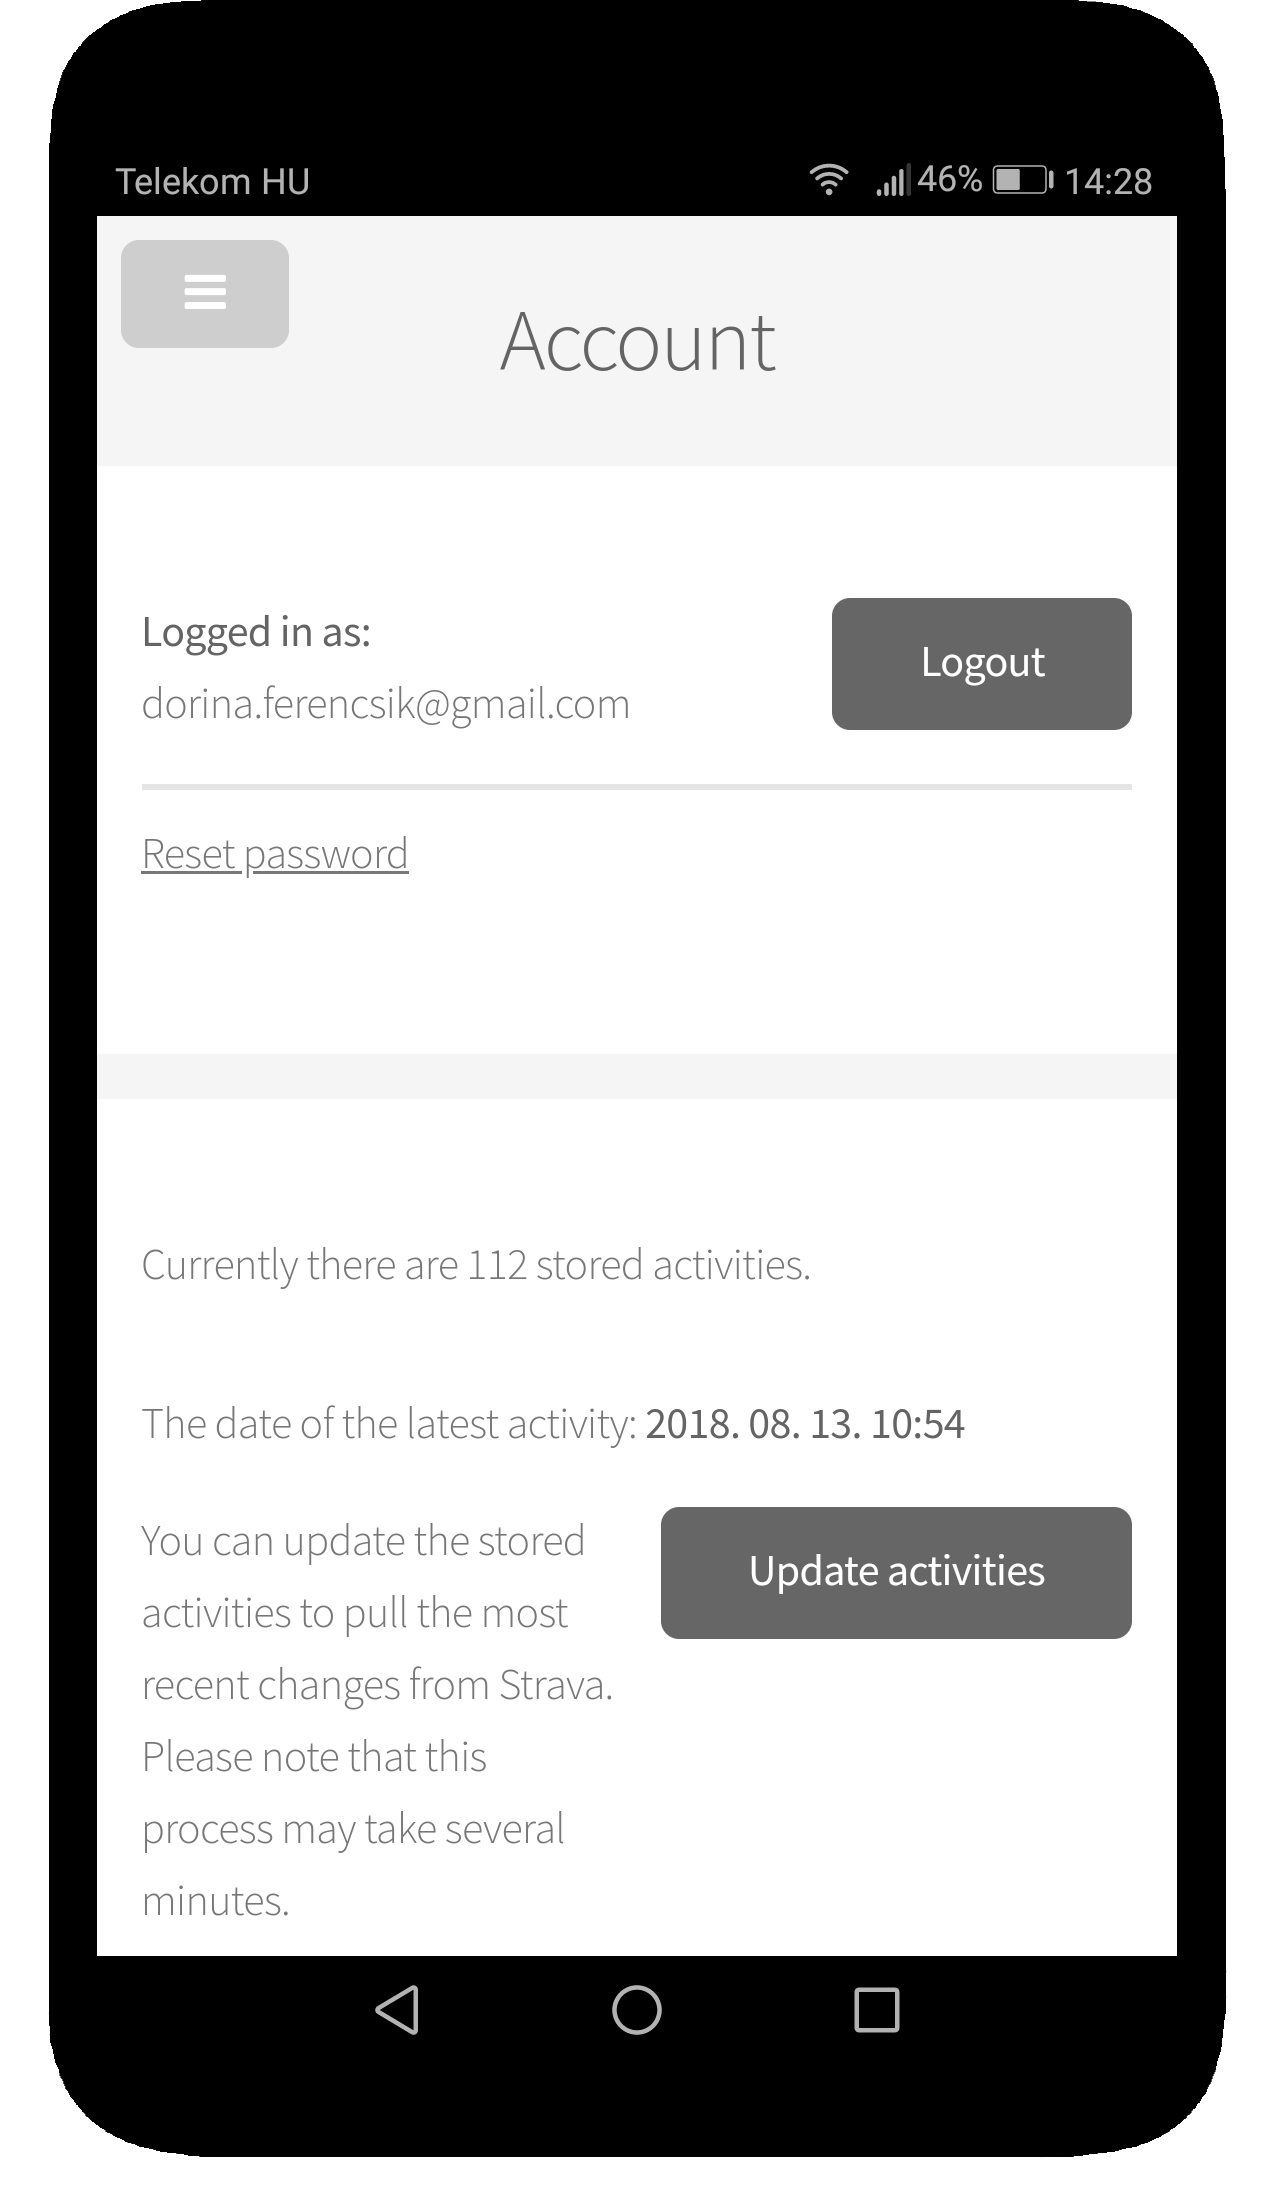
\includegraphics[ width=\textwidth,keepaspectratio]{kepek/website/websiteAccount.png}
		\caption{Fiók}
		\label{fig:websiteAccount}
	\end{subfigure}
	
	\caption{Adatgyűjtő weboldal alapvető funkciói}
%	\label{fig:websiteRegister}
\end{figure}

\subsubsection{JQuery}
A JQuery \cite{jquery} egy népszerű JavaScript könyvtár amely lehetőséget ad a HTML elemek könnyebb manipulálására, az események egyszerűbb kezelésére, animációk megvalósítására. 

\subsubsection{Firebase}
A Firebase \cite{firebase} egy Google által fejlesztett sokoldalú rendszer, amely egyszerű eszközöket kínál egy weboldal logikai részének felépítéséhez. Nem alkalmas robosztus rendszerek létrehozásához, azonban kisebb projektek menedzseléséhez megfelelő alapot kínál. A projekteket létrehozás után online lehet kezelni és a Firebase funkcióit weboldalakban és mobil alkalmazásokban is (mind Android és iOS) egyszerűen lehet használni. A rendszer alapját egy Node.js szerver és egy JSON alapú adatbázis adja valamint elérhető egy általános célú tárhely tetszőleges file-ok tárolásához. 

\subsubsection{Firebase - Autentikáció}
A szakdolgozathoz készített weboldal szempontjából a Firebase egyik legfontosabb eleme az autentikációs rendszer. A Firebase felületén való engedélyezés után a weboldal kódbázisában gyorsan és biztonságosan megvalósítható az új felhasználók regisztrálása, bejelentkeztetése. Az email alapú regisztráláson túl lehetőség van külső rendszerekkel való autentikációra is mint a Google fiók, Facebook, Github. Továbbá elérhető a már regisztrált felhasználók emailen keresztül történő értesítése is.

\subsubsection{Firebase - Adatbázis}
A Firebase alapvetően ingyenes, emiatt az adatbázisnak vannak méret és sebességbeli korlátjai, azonban megfelelő kiindulási alapot ad. A JSON alapú struktúra megkönnyíti az adatok kliens oldalon történő kezelését valamint egy ilyen méretű alkalmazás esetén egyszerűen karban tartható. Fontos kiemelni az adatbázis hozzáférhetőségének konfigurálási lehetőségét. Lehetőség van az adatbázis egészére vagy a részfákra olvasási és írási beállításokat megadni, amik korlátozhatóak a bejelentkezett felhasználó azonosítója alapján is. Ennek felhasználásával könnyen megvalósítható hogy a rendszer összes felhasználója csak a saját adataihoz férjen hozzá ami fontos adatvédelmi szempont.

\SubSection{Adatstruktúra} \label{ssec:adatstruktura}
A szakdolgozathoz készített weboldal fő célja hogy lekérje és tárolja azon felhasználók útvonalait akik regisztrálás után kapcsolódtak a Strava fiókjukhoz. A Strava API-ja az utak lekérésekor SummaryActivity objektumok tömbjével tér vissza, ahol minden objektum 39 változóval jellemez egy utat, aktivitást. Ez a 39 jellemző magába foglalja többek között a felhasználó azonosítóját, a megtett távot, a teljesített kihívások számát, az ismerősök megjegyzéseinek a számát és rengeteg egyéb információt. A gépi tanulás során ezeknek a jellemzőknek csak egy részét érdemes használni, amik szorosabban kapcsolódnak az út valós leírásához. Ezek a jellemzők valamit a felhasználókhoz kapcsolódó adatok szerkezete a \myref{fig:dataStructure} ábrán látható, leírásuk a következőkben kerül részletezésre.

\begin{figure}[!h]
	\centering
	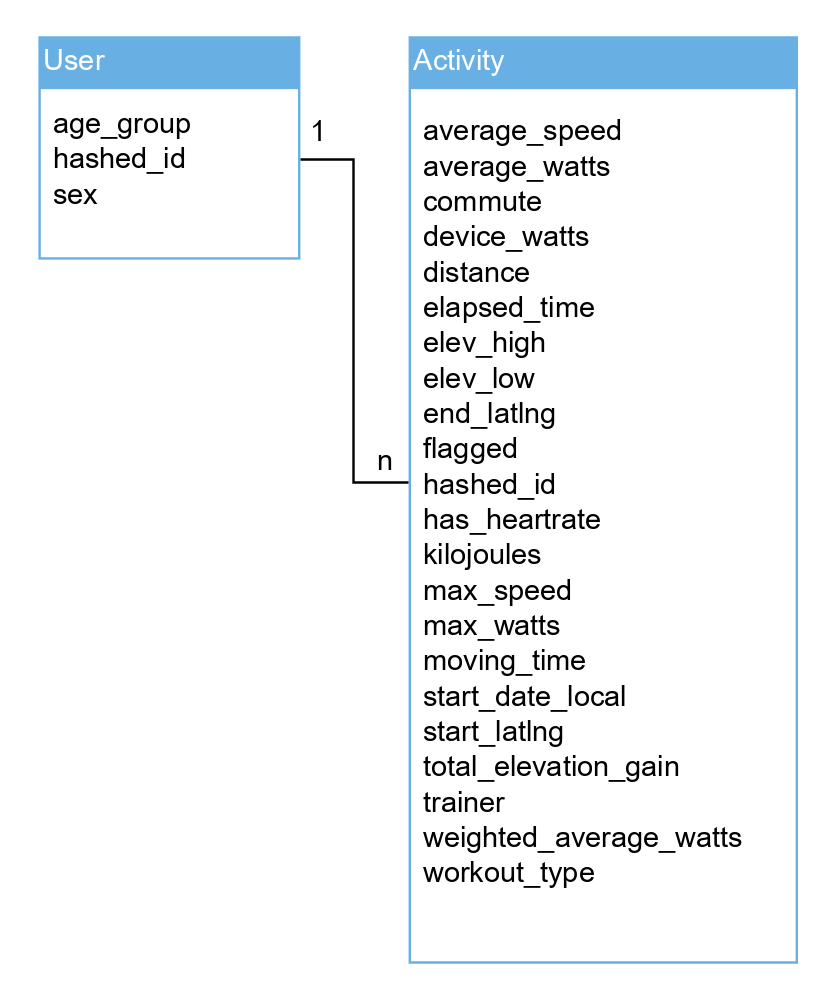
\includegraphics[ width=0.7\textwidth,keepaspectratio]{kepek/data_structure.png}
	\caption{Adatstruktúra}
	\label{fig:dataStructure}
\end{figure}

\noindent \textbf{Jellemzők magyarázata:}
\begin{itemize}
	\item \textbf{age\_group: } felhasználó korcsoportja (0: 18-30; 1: 31-45; 2: 45+)
	\item \textbf{hashed\_id:} felhasználó azonosító hash-elt változata
	\item \textbf{sex: } felhasználó neme (male / female, férfi / nő)
	\item \textbf{average\_speed:} átlagsebesség (méter/másodperc)
	\item \textbf{average\_watts:} átlagos erőkifejtés az útvonal során. Amennyiben nem biztosított az értéke -1
	\item \textbf{commute:} egy tevékenység rögzítésekor lehetőség van azt 'ingázásként' felcímkézni, ezzel megjelölve hogy nem egy verseny vagy túra adat, hanem mindennapi, például munkába vagy boltba járási útvonal. Feltételezhető hogy ilyenkor az illető nem a minél jobb eredmények elérésére törekszik, inkább rutin szerűen, átlagos tempóban halad (logikai; -1 amennyiben nem biztosított)
	\item \textbf{device\_watts:} azt jelöli hogy az erőkifejtési adatokat tényleges mérőkészülék szolgáltatja vagy csupán becsült érték (logikai; Hamis amennyiben becsült érték) 
	\item \textbf{distance:} a megtett távolság (méter)
	\item \textbf{elapsed\_time:} összesen eltelt idő (másodperc)
	\item \textbf{elev\_high:} az út legmagasabb pontja (méter)
	\item \textbf{elev\_low:} az út legalacsonyabb pontja (méter)
	\item \textbf{end\_latlng:} az útvonal végpontjának hosszúsági és szélességi helyzete
	\item \textbf{flagged:} az útvonal meg van e jelölve (logikai)
	\item \textbf{has\_heartrate:} elérhető e pulzus adat (logikai)
	\item \textbf{kilojoules:} összes kifejtett erő mennyisége (kilojoule)
	\item \textbf{max\_speed:} maximum sebesség az út során (méter/másodperc)
	\item \textbf{max\_watts:} maximális erőkifejtés az út során
	\item \textbf{moving\_time:} mozgással töltött idő (másodperc)
	\item \textbf{start\_date\_local:} az út kezdési ideje (dátum)
	\item \textbf{start\_latlng:} az útvonal kezdőpontjának hosszúsági és szélességi helyzete
	\item \textbf{total\_elevation\_gain:} összesen megtett emelkedő (méter)
	\item \textbf{trainer:} az útvonal gépen lett e megtéve (logikai)
	\item \textbf{weighted\_average\_watts:} súlyozott átlagos erőkifejtés az útvonal során. Ha  nem biztosított az értéke: -1.
	\item \textbf{workout\_type:} tevékenység típusa, lehet edzés vagy verseny (egész szám, ha nincs megadva akkor -1. Lehetséges értékei: 10 - normál kerékpározás; 11 - verseny; 12 - edzés )
\end{itemize}












\Chapter{Fejlesztői dokumentáció}
\label{Chap:dokumen}

\iffalse
Ebben a fejezetben kell a hallgatónak leírnia a saját eredményeit. Például ilyennek tekinthető a hallgató által elkészített program leírása, algoritmus leírása alkalmazási lehetőségek, eredmények. Lehet benne több alfejezet vagy al-alfejezet is. Ezek számozása és a tartalomjegyzékben  való megjelenítése rögzített. A fejezet címe megváltoztatható az eredmények szerint. Ez a fejezet és a \aref{Chap:tema} együtt összesen 25-60 oldal terjedelmű kell hogy legyen
\fi

Az Elméleti kifejtés során meghatározott célokat különböző gépi tanulási módszerekkel lehet megoldani amik eltérő eredménnyel, pontossággal fognak működni. A nehézségi osztályok meghatározására elsősorban a  \myaref{ssec:klaszterezes} pontban részletezett klaszterezési módszerek használhatóak

\Section{Adathalmaz előkészítés}
A fejlesztés legelső lépése az összegyűjtött adatok megfelelő struktúrára való átalakítása és megtisztítása, ezzel megkönnyítve a későbbi feldolgozást valamint növelve a gépi tanulási algoritmusok pontosságát

\SubSection{Adatstruktúra kialakítása}
Az adatgyűjtés elsődleges eszközeként a szakdolgozat keretein belül készített weboldal szolgált, amely minden információt egy JSON alapú adatbázisban tárolt le. Az adathalmaz előkészítésének a legelső lépése a JSON struktúráról való áttérés egy, a Python programozási nyelv által kezelt, könnyen használható adatstruktúrára. Erre a szakdolgozat során a Pandas \cite{python-pandas} nevű Python csomag által megvalósított DataFrame nevű struktúra fog szolgálni , amely segítségével az adatokat táblázathoz hasonló formában lehet tárolni. Egy DataFrame oszlopai egyedi, a fejlesztő által definiált oszlopnevekkel érhetőek el, soraira index használatával lehet hivatkozni. Az oszlopok egyenként különböző típusúak lehetnek és tartalmazhatnak NULL értékeket. A DataFrame egyik legnagyobb előnye az oszlopok nevesítése, amivel könnyen nyomon követhető hogy az aktuális értékek melyik feature-nek felelnek meg, mit reprezentálnak a valóságban

\begin{programreszlet}
A  parancs segítségével a JSON struktúra (jsonData) könnyen átalakítható DataFrame-é (dataset). A dataset oszlopai megfelelnek a \myaref{ssec:adatstruktura} pontban részletezett adatoknak.
\begin{python}
import pandas

jsonData = pandas.read_json("2019_03_20_10h.json", type='series')
cleanData = []
for u in userData:
  if userData[u]['connectedToStrava'] == True:
    for i in range(0,len(userData[user]['activities'])):
       userData[u]['activities'][i]['ageGroup'] = userData[u]['ageGroup']
       userData[u]['activities'][i]['sex'] = userData[u]['sex']
       userData[u]['activities'][i].pop('external_id', None)
       userData[u]['activities'][i].pop('map_id', None)
       userData[u]['activities'][i].pop('map_resource', None)
       userData[u]['activities'][i].pop('map_summary', None)
       cleanData.append(userData[u]['activities'][i]) 
  else:
    print('User does not have any activities')
dataset = pandas.DataFrame(cleanData)

\end{python}
\end{programreszlet}


A fenti parancs segítségével a JSON struktúra (jsonData) könnyen átalakítható DataFrame-é (dataset). A dataset oszlopai megfelelnek a \myaref{ssec:adatstruktura} pontban részletezett adatoknak.


\SubSection{Adattisztítás}
A megfelelő adatstruktúra kialakítása után a következő lépés az adatok megtisztítása. Ez a lépés azért szükséges mert a legfigyelmesebben gyűjtött adathalmaz is tartalmazhat rossz értékeket illetve előfordulhat hogy több helyen hiányzik a valódi érték. Ezeknek a hibáknak a megtalálása és kijavítása több fázisból áll.

%\csvautotabular{adat/rawDataDescription.csv}
A megtaláláshoz első lépés az adatok áttekintése: NULL értékek vizsgálata, egyes jellemzők eloszlásának megtekintése, minimum, maximum és a kvantilisek összehasonlítása. Ehhez nyújt segítséget a \myref{tab:rawDataDescription} táblázat amely a numerikus oszlopokról készült általános jellemzést összegzi. 
\begin{table}[!h]
	\resizebox{\textwidth}{!}{%
		\begin{tabular}{l|l|l|l|l|l|l|l|l|}
			\cline{2-9}
			& \multicolumn{1}{c|}{\textbf{Count}} & \multicolumn{1}{c|}{\textbf{Mean}} & \multicolumn{1}{c|}{\textbf{STD}} & \multicolumn{1}{c|}{\textbf{Min}} & \multicolumn{1}{c|}{\textbf{0.25}} & \multicolumn{1}{c|}{\textbf{0.50}} & \multicolumn{1}{c|}{\textbf{0.75}} & \multicolumn{1}{c|}{\textbf{Max}} \\ \hline
			\multicolumn{1}{|l|}{
				\textbf{age\_group}}  & 10014  & 1.01   & 0.48   & 0.0   & 1.0   & 1.0   & 1.0   & 2.0   \\ \hline
			\multicolumn{1}{|l|}{
				\textbf{average\_speed}}  & 10014   & 24.25   & 653.31  & 0.0  & 4.96   & 5.73  & 6.47  & 36100.0  \\ \hline
			\multicolumn{1}{|l|}{
				\textbf{average\_watts}}  & 1848  & 163.0  & 49.51  & 0.0  & 139.10  & 161.85  & 180.85 & 482.6 \\ \hline
			\multicolumn{1}{|l|}{
				\textbf{distance}} & 10014  & 26153.09 & 29465.23 & 0.0   & 7444.83 & 13751.25 & 34587.2  & 436806.0  \\ \hline
			\multicolumn{1}{|l|}{
				\textbf{elapsed\_time}} & 10014 & 5845.88 & 19296.2  & 0.0  & 1648.00  & 3020.0  & 7343.0  & 1806211.0  \\ \hline
			\multicolumn{1}{|l|}{
				\textbf{elev\_high}} & 9845 & 282.1 & 272.66 & -71.2  & 162.2  & 229.4  & 296.4 & 12103.0  \\ \hline
			\multicolumn{1}{|l|}{
				\textbf{elev\_low}}  & 9844  & 131.99 & 68.68  & -500.0  & 103.1 & 130.0 & 148.3  & 1484.0 \\ \hline
			\multicolumn{1}{|l|}{
				\textbf{kilojoules}} & 1765 & 1295.76 & 756.06 & 0.0 & 728.7 & 1236.7 & 1745.4  & 5928.8   \\ \hline
			\multicolumn{1}{|l|}{
				\textbf{max\_speed}} & 10014  & 12.14 & 3.99  & 0.0  & 9.6 & 11.6  & 14.48  & 122.7        \\ \hline
			\multicolumn{1}{|l|}{
				\textbf{max\_watts}} & 546 & 630.95  & 244.34  & 115.0 & 502.0 & 603.0  & 708.0 & 2428.0   \\ \hline
			\multicolumn{1}{|l|}{
				\textbf{moving\_time}}  & 10014  & 4543.18  & 5016.52  & 0.0 & 1442.0  & 2451.0  & 6109.0  & 90983.0  \\ \hline
			\multicolumn{1}{|l|}{
				\textbf{pr\_count}}  & 1959  & 1.48  & 3.2 & 0.0 & 0.0 & 0.0  & 2.0   & 50.0       \\ \hline
			\multicolumn{1}{|l|}{
				\textbf{resource\_state}}  & 1959  & 2.0  & 0.0  & 2.0  & 2.0  & 2.0  & 2.0  & 2.0                \\ \hline
			\multicolumn{1}{|l|}{
				\textbf{\begin{tabular}[c]{@{}l@{}}total\_elevation\\ \_gain\end{tabular}}}  & 10014  & 278.7  & 428.88  & 0.0  & 27.5   & 85.2 & 361.8   & 4416.8   \\ \hline
			\multicolumn{1}{|l|}{
				\textbf{\begin{tabular}[c]{@{}l@{}}weighted\_average\\ \_watts\end{tabular}}} & 546  & 188.86  & 30.35  & 5.0   & 176.25  & 195.0  & 208.75  & 246.0  \\ \hline
			\multicolumn{1}{|l|}{
				\textbf{workout\_type}}  & 4039    & 9.74   & 1.85   & 0.0  & 10.0  & 10.0  & 10.0    & 12.0 \\ \hline
		\end{tabular}%
	}
\caption{Nyers adathalmaz leírás}
\label{tab:rawDataDescription}
\end{table}

A táblázat oszlopainak a jelentése:
\begin{itemize}
	\item Count: adott jellemző nem NULL értékeinek darabszámát adja meg
	\item Mean: adott jellemző átlaga
	\item STD (Standard Deviation): adott jellemző szórása
\end{itemize}



\subsubsection{NULL értékek}
Egy általános adatbázis esetén gyakran előfordul hogy egyes oszlopok NULL értékeket tartalmaznak - ebben az esetben például NULL jelöli ha egy útvonal nincs elérhető adat egy adott jellemzőről. Azonban a gépi tanulási algoritmusok számokat képesek feldolgozni így elengedhetetlen a NULL értékek kiküszöbölése valamilyen formában.

A NULL értékek kiküszöbölésére két elterjedt megoldás létezik:
\begin{itemize}
	\item \textbf{NULL értékek törlése:} az egyszerűbb megoldás a NULL értékeket tartalmazó sorok törlése, azonban ennek a módszernek nagy hátránya hogy sok NULL-t tartalmazó adathalmaz esetén jelentős mértékben megcsappan az adathalmaz mérete
	\item \textbf{NULL értékek feltöltése:} összetettebb, azonban sok esetben célravezetőbb megoldást jelent a NULL értékek helyettesítése valamilyen számított értékkel. Az új értékek számítása különböző módokon történhet, ez nagyban függ az adott jellemző jellegétől
\end{itemize}
Amennyiben egy oszlop nagy mértékben tartalmaz NULL értékeket érdemes megfontolni az elvetését vagy külön esetként kezelni mikor van tényleges érték

Az adat vizsgálata után az első szembetűnő gond a hiányzó értékek. Az alábbi jellemzők akkora mértékben hiányosak hogy a javításuk reménytelen feladat, így az adattisztítás elején törlésre kerültek.
\begin{itemize}
	\item average\_watts: 18.45\% hasznos értéket tartalmaz
	\item commute: 98.83\% hasznos értéket tartalmaz azonban ezekből csupán 23 True érték
	\item device\_watts : 19.56\%
	\item flagged : 19.56\%
	\item has\_heartrate : 19.56\%
	\item heartrate\_opt\_out: 
	\item kilojoules : 17.63\%
	\item max\_watts 5.54\%
	\item pr\_count : 19.56\%
	\item resource\_state : 19.56\%
	\item weighted\_average\_watts : 5.45\%
	\item sex : 100\% hasznos azonban elenyészően kevés női adatot tartalmaz az adathalmaz, ezért a torzítatlanság érdekében a szakdolgozat során csak a férfi útvonalak kerülnek felhasználásra - így ez az jellemző funkcióját veszti, konstans érték
	\item start\_latlng : 18.34\%
	\item end\_latlng : 18.34\%
\end{itemize}


\subsubsection{Kiugró értékek}
Gyakori jelenség hogy egy jellemző tartalmaz néhány magasan kiugró értéket, amelyek sokszor érvényesek azonban fakadhatnak mérési / rögzítési hibából is. Akár érvényes értékek, akár valamilyen hibából erednek érdemes kiküszöbölni őket mivel könnyen eltorzíthatják az eredményeket. 

A kiugró értékek megtalálása egy alapvető módszer került felhasználásra a szakdolgozat készítése során. A kiugró értékeket jellemzőként külön vizsgáljuk. $F$ jellemzőre $x \in F$ érték kiugrónak tekinthető amennyiben

\[  \frac{x - \overline{F}}{\sigma} > 2.5\]
teljesül, ahol $\overline{F}$ az $F$ jellemző átlaga, $\sigma$ pedig $F$ szórása.

Az alábbiakban a különböző jellemzők kiugró érték vizsgálatának részletes leírása található.\\[6pt]

\textbf{Átlagsebesség (average\_speed):}
ez a jellemző m/s-al adja meg az útvonal átlagsebességét. A fenti módszer 10 kiugró értéket talált amik 2182 m/s (7855.2 km/h) és 28290 ms/s (101844.0 km/h) közé esnek. Ekkora sebesség elérése nyilvánvalóan lehetetlen kerékpárral, eredetük az adatsorok megvizsgálása után leszűkíthető a mozgási idő (moving\_time) jellemző mérésének a hiányára / hibájára. Az átlagsebesség számítása ugyanis a távolság és a mozgási idő hányadosaként kerül kiszámításra és a vizsgált kiugró értékeknél a mozgási idő mindenhol 1 másodperc míg a távolság 10 km fölött van. Ezen adatok javítása nem tűnik megvalósíthatónak. Eldobásuk után az adathalmaz 10004 utat tartalmaz.\\[6pt]

\textbf{Távolság (distance):}
a distance jellemző méterben megadva tárolja az egy-egy útvonal során megtett távolságot. Kiugró érték vizsgálat során 313 értéket talált a módszer, amik között a legkisebb értéke 99915.1 méter azaz közel 100 km. Ezek az adatsorok azonban minden más szempontból helyes értékeket tartalmaznak és valójában a 100 km-s utak sem lehetetlenek. Ezek az értékek nem kerültek törlésre az adathalmazból azonban a későbbiek során érdemes lehet a hasonlóan hosszú utakat külön kezelni\\[6pt]

\textbf{Legmagasabb tengerszint feletti pont (elev\_high):}
az elev\_high jellemző vizsgálata során 61 kiugró érték jelzett a módszer amelyek 976.6 méter és 12103.0 méter közé esnek. A 12103 méter egyértelműen lehetetlen, a többi érték pedig vele együtt elvetésre kerül. Ezen adatsorok eldobása után az adathalmaz 9943 útvonalat tartalmaz\\[6pt]

\textbf{Legnagyobb sebesség (max\_speed)}
a max\_speed az útvonal során mért maximális sebességet jelzi m/s mértékegységben. Vizsgálata során a használt módszer 218 kiugró értéket talált. Ezek az értékek két intervallumra oszthatóak fel. 0.0 m/s - 2.1 m/s és 22.1 m/s - 122.7 ms azaz 0.0 km/h - 7.56 km/h és 79.56 km/h - 441.72 km/h. Ezek olyan adatok amelyek kilógnak az adathalmazból, sok közülük lehetetlen / értelmezhetetlen. Ezen adatsorok eldobása után az adathalmaz 9725 útvonalat tartalmaz.\\[6pt]

\textbf{Mozgási idő (moving\_time)}
a moving\_time jellemző a tényleges mozgással töltött időt tárolja másodpercben megadva. A jellemző vizsgálata során 276 érték bizonyult kiugrónak amelyek közül a legkisebb értéke 16814 másodperc azaz nagyjából 4 óra és 40 perc. Ezek az értékek összefüggnek a távolság (distance) jellemző vizsgálata során talált kiugró értékekkel, így egyenlőre az adathalmaz része marad, a későbbiek során azonban külön lesz kezelve.


A kiugró értékek megtalálására használt módszeren felül definiálásra került néhány szabály amik segítségével ki lehet szűrni az egyéb helytelen adatokat. Ezek alapján elvetésre kerülnek azok az adatsorok ahol:
\begin{itemize}
	\item az átlagsebesség kisebb mint 2 m/s (7.2 km/h)
	\item a távolság kisebb mint 100 méter (néhány száz méter esetén előfordulhat hogy rövid sprinteket tettek meg a sportolók)
	\item a legmagasabb vagy legalacsonyabb tengerszint feletti magasság hiányzó adat
\end{itemize} 
Továbbá 2 helyen javításra került az összes eltelt idő (elapsed\_time) mivel kevesebb volt mint a mozgással tölött idő (moving\_time)


A fentebbi adatsorok eldobása után összességében 9603 útvonalat tartalmazó adathalmaz maradt.


\SubSection{Adatok áttekintése}
A további feldolgozás illetve a tényleges gépi tanulási algoritmusok felhasználása előtt érdemes kicsit mélyrehatóbban tanulmányozni az adathalmazt, felfedezni a mintákat és összefüggéseket. 



\begin{figure}
	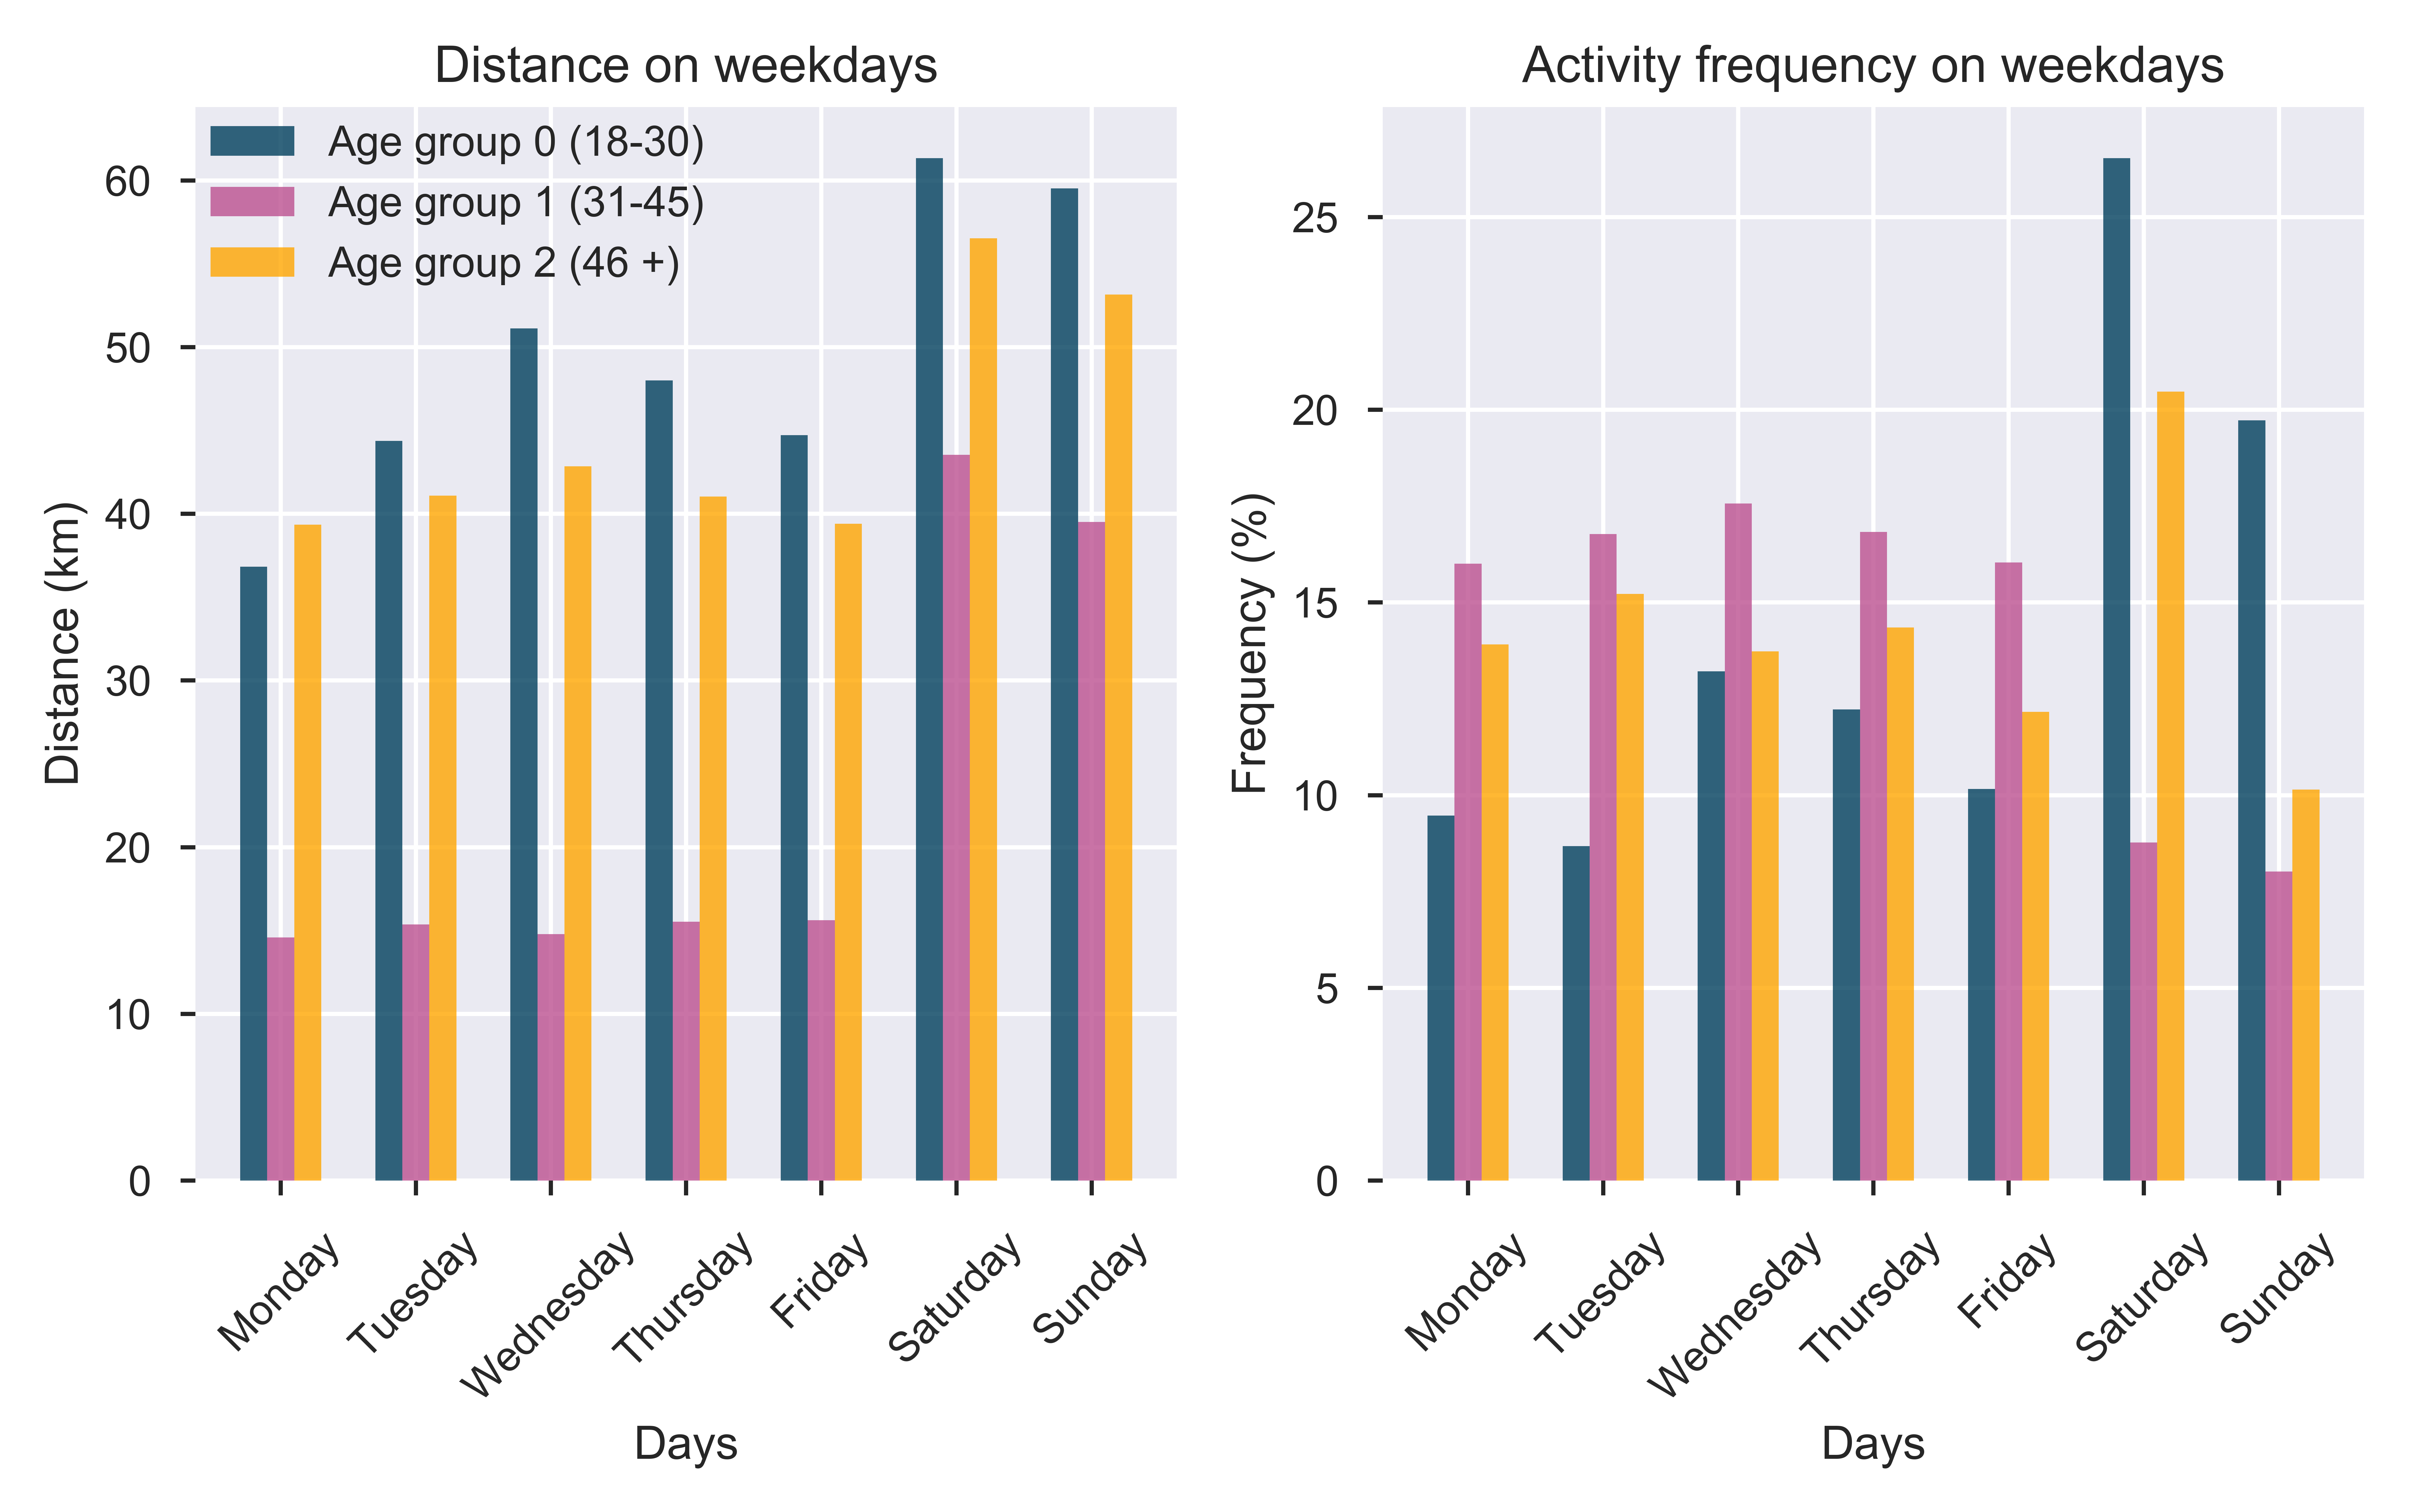
\includegraphics[width=\linewidth]{kepek/FrequencyAndDistanceOnWeekDays.png}
	\caption{Átlagos távolság és útvonal gyakoriság a hét napjain}
	\label{fig:distanceAndFrequencyByWeekdays}
\end{figure}

A \myref{fig:distanceAndFrequencyByWeekdays} ábrán két grafikon jellemzi az útvonalak eloszlását a hét napjai szerint. A bal oldali gráfon az átlagosan megtett távolságot, a jobb oldali pedig az útvonalak darabszámának eloszlását jelzi, korcsoportok szerint lebontva.


Szöveg a fenti képről....

Blablabla

Még mindig.....


\begin{figure}[!h]
	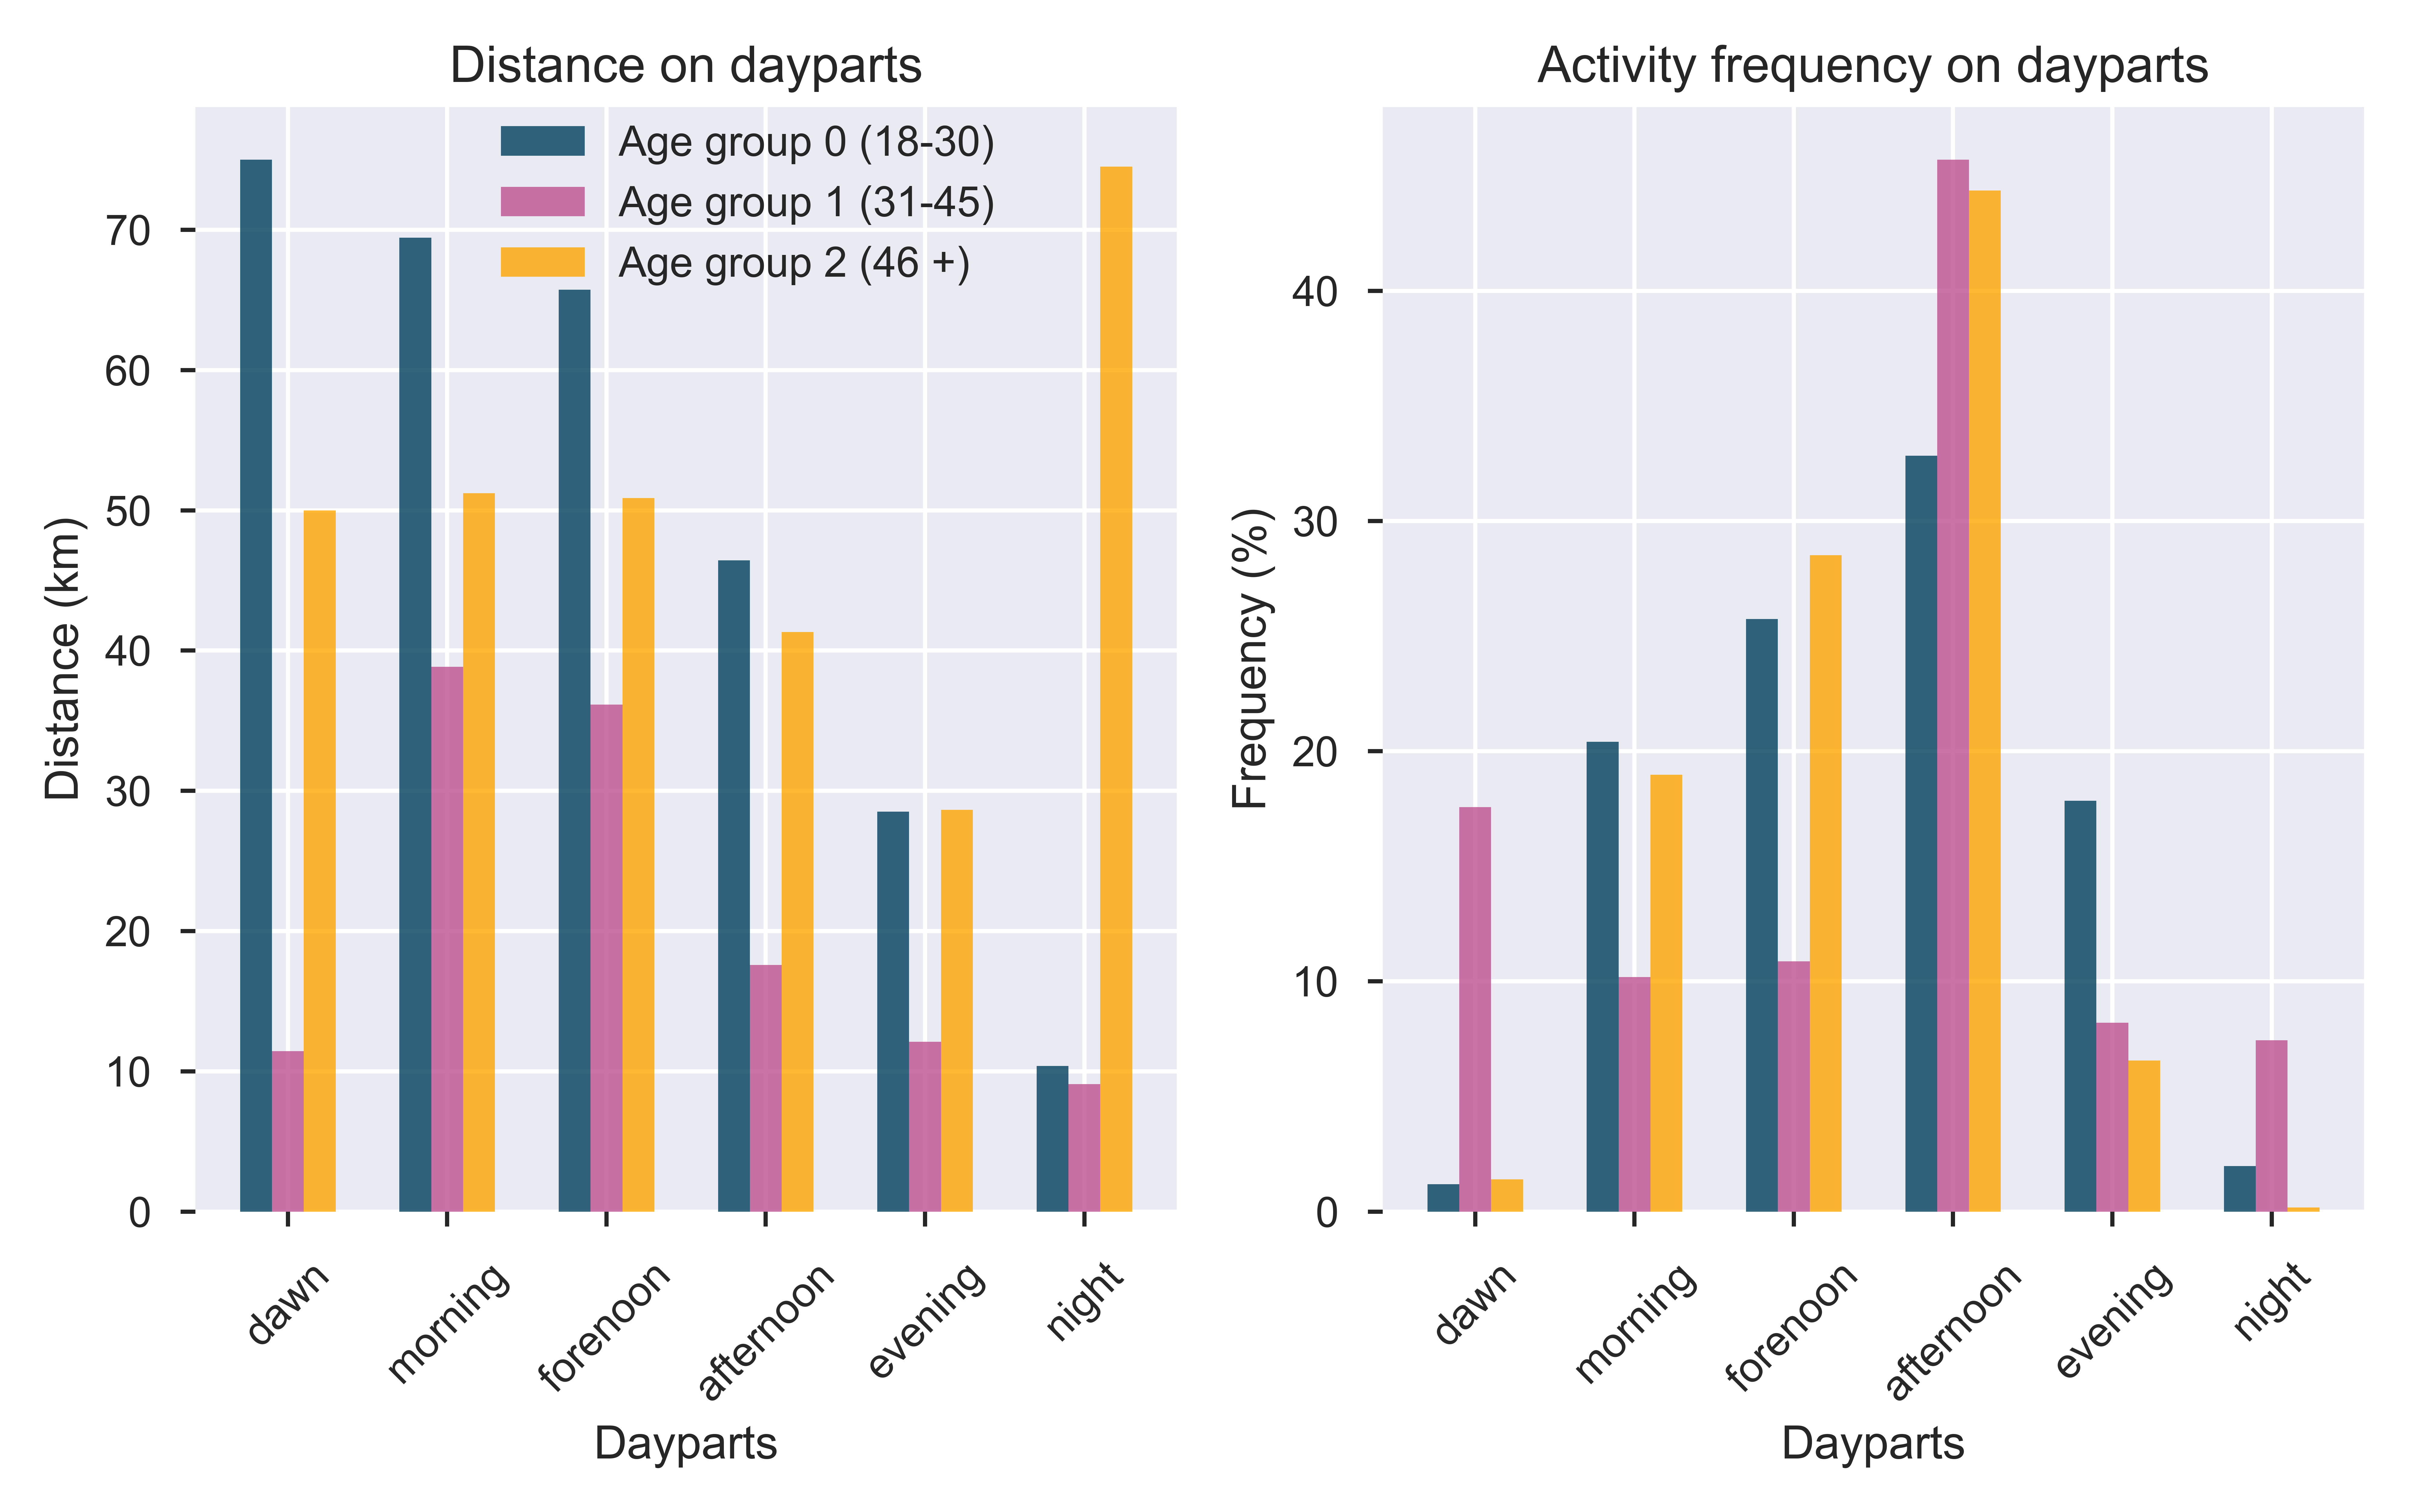
\includegraphics[width=\linewidth]{kepek/FrequencyAndDistanceOnDayparts.png}
	\caption{Átlagos távolság és útvonal gyakoriság napszakok szerint}
	\label{fig:distanceAndFrequencyByDayparts}
\end{figure}








\SubSection{További adat feldolgozás}

\subsubsection{One-hot encoding}
A kiugró értékek kezelése és a adathalmaz összefüggéseinek vizsgálata után a következő lépés a one-hot encoding. Az eljárás lényege hogy egy kategória alapú jellemzőt több (a kategóriák számának megfelelő) oszlopra bont szét, ahol az egyes oszlopokban, jellemzőkben 1-es szerepel amennyiben az adatsor abba az adott kategóriába sorolható, 0 egyébként. Ennek az előnye hogy kiküszöböli a kategóriák sorszámmal történő jelzésének távolságát. Például egy korcsoportot tároló jellemző esetén nem biztos hogy helyes feltételezni hogy a 0. és a 2. kategória (csoport) között 2 távolság van. A one hot encoding természetesen folytonos változók esetén nem értelmezhető és kategoriális jellemzőkre sem mindig érdemes alkalmazni.

A szakdolgozathoz használt adathalmaz esetén 3+1 jellemző kerül one-hot encode-olásra: age\_group (korcsoport), workout\_tpye, start\_date\_local és a training.\\[6pt]

\textbf{age\_group:} a sportoló korcsoportját jelzi, értékei egy három elemű halmazból kerülhetnek ki: \{0, 1, 2\} ahol 0 a [18,30], 1 a [31,45], 2 pedig a [46,$+\infty$) korcsoportokba való tartozást jelenti. One-hot encoding során az eredeti jellemzőből 3 oszlop készül, végül az eredeti törlésre kerül az adathalmazból.
\begin{programreszlet}
Python parancsok részletezése
\begin{python}
ageOneHot = pandas.get_dummies(rawData['age_group'], prefix='age')
rawData.drop(columns=['age_group'], inplace=True)
rawData = rawData.join(ageOneHot)
\end{python}
\end{programreszlet}
A kódban megadott prefix paraméter segítségével az új jellemzők nevei: age\_0.0, age\_1.0, age\_2.0\\[6pt]


\textbf{workout\_tpye:} 

\begin{programreszlet}
	\TODO szöveg
\begin{python}
workoutTypeOneHot = pandas.get_dummies(rawData['workout_type'],
				       prefix='workout_type')
rawData.drop(columns='workout_type', inplace=True)
rawData = rawData.join(workoutTypeOneHot)
\end{python}
\end{programreszlet}


\textbf{start\_date\_local:} a jellemző az aktivitás kezdeti idejét tárolja, a sportoló saját időzónája szerint, ÉÉÉÉ-MM-DD HH:MM:SS formátumban. Dátum mezők azonban nem értelmezhetőek gépi tanulási algoritmusokkal így a jellemző átalakítása szükségszerű volt. A dátumból alapvetően 2 féle új jellemző kerül kinyerésre, majd ezek külön kerülnek one-hot encode-olásra

\begin{programreszlet}
Az aktivitás kezdetének dátumából kinyerhető hogy a hét melyik napján történt az aktivitás. Ezen információ kinyerését és one-hot encode-olását az alábbi kód végzi
\begin{python}
rawData['day_of_week'] = rawData['start_date_local'].dt.day_name()
weekDayOneHot = pandas.get_dummies(rawData['day_of_week'], 
				   prefix='weekday')
rawData.drop(columns=['day_of_week'], inplace=True)
rawData = rawData.join(weekDayOneHot)
\end{python}		
\end{programreszlet}

\begin{programreszlet}
Az aktivitás kezdetének időpontjából kinyerhető hogy melyik napszakban kezdődött az aktivitás. Ezen információ kinyerését és one-hot encode-olását az alábbi kód végzi
\begin{python}
rawData['daypart'] = rawData['start_date_local'].apply(lambda row: 
						 timeToPartOfDay(row))
dayPartOneHot = pandas.get_dummies(rawData['daypart'], prefix='daypart')
rawData.drop(columns=['daypart'], inplace=True)
rawData = rawData.join(dayPartOneHot)
\end{python}	

Ahol a timeToPartOfDay függvény a start\_date\_local jellemző minden adattagjára külön hívódik meg. Ez a függvény szubjektíven oszt fel egy napot hat napszakra \myaref{fig:daypartsClock} ábra szerint

\end{programreszlet}

\begin{figure}[!h]
	\centering
	\begin{tikzpicture}[line cap=rect,line width=3pt]
	\filldraw[fill=chart5, draw=chart5, line width=1pt] (0,0)-- +(45:2) arc (45:0:2); %hajnal
	\filldraw[fill=chart0, draw=chart0, line width=1pt] (0,0)-- +(120:2) arc (120:45:2); %éjszaka
	\filldraw[fill=chart1, draw=chart1, line width=1pt] (0,0)-- +(180:2) arc (180:120:2); %este
	\filldraw[fill=chart2, draw=chart2, line width=1pt] (0,0)-- +(270:2) arc (270:180:2); %délután
	\filldraw[fill=chart3, draw=chart3, line width=1pt] (0,0)-- +(315:2) arc (315:270:2); %délelőtt
	\filldraw[fill=chart4, draw=chart4, line width=1pt] (0,0)-- +(360:2) arc (360:315:2); %reggel
	
	\node[font=\small] at (90:2.36cm) {\textsf{Éjszaka}};
	\node[font=\small] at (20:2.7cm) {\textsf{Hajnal}};
	\node[font=\small] at (340:2.7cm) {\textsf{Reggel}};
	\node[font=\small] at (305:2.6cm) {\textsf{Délelőtt}};
	\node[font=\small] at (215:2.7cm) {\textsf{Délután}};
	\node[font=\small] at (155:2.6cm) {\textsf{Este}};
	
	\draw (0,0) circle [radius=2cm];
	
	\foreach \angle [count=\xi] in {75,60,...,-270}
	{
		\draw[line width=1pt] (\angle:1.8cm) -- (\angle:2cm);
		%\node[font=\small] at (\angle:1.36cm) {\textsf{\xi}};
	}
	\foreach \angle [count=\xi] in {0,45,90,135,180,225,270,315}
	{
		\draw[line width=2pt] (\angle:1.6cm) -- (\angle:2cm);
	}
	\draw (0,0) -- (120:0.8cm);
	\draw (0,0) -- (90:1cm);
	\node[font=\small] at (0:1.36cm) {\textsf{6}};
	\node[font=\small] at (45:1.36cm) {\textsf{3}};
	\node[font=\small] at (90:1.36cm) {\textsf{0}};
	\node[font=\small] at (135:1.30cm) {\textsf{21}};
	\node[font=\small] at (180:1.36cm) {\textsf{18}};
	\node[font=\small] at (225:1.36cm) {\textsf{15}};
	\node[font=\small] at (270:1.36cm) {\textsf{12}};
	\node[font=\small] at (315:1.36cm) {\textsf{9}};
	
	
	%\filldraw[line color=gray!40 ] -- +(45:2) arc (45:-45:2);
	\end{tikzpicture}
	\caption{Napszakok kialakítása.}
	\label{fig:daypartsClock}
\end{figure}

\textbf{trainer: } a trainer jellemző Igaz / Hamis értékekkel jelzi hogy egy adott aktivitás traineren, azaz gépen történt e, nem pedig tényleges kerékpáron. Ennek a jellemzőnek az átalakítása nem igazi one-hot encoding, inkább csak az Igaz / Hamis értékek átalakítása 1 / 0 értékekre.  


Az adattisztítás összes lépése után az adathalmaz szerkezete lényegesen megváltozik, új jellemzőket tartalmaz (one-hot encoding) valamint az eddigi jellemzők sok esetben más intervallumokba esnek (kiugró értékek kezelése).

Jellemzők:
\begin{itemize}
	\item average\_speed
	\item distance
	\item elapsed\_time
	\item elev\_high
	\item elev\_low
	
	\item hashed\_id 
	\item max\_speed
	\item moving\_time
	\item total\_elevation\_gain
	\item age\_0.0 
	\item age\_1.0
	\item age\_2.0
	\item trainer\_onehot
	\item workout\_type\_0.0
	\item workout\_type\_4.0 
	\item workout\_type\_10.0 
	\item workout\_type\_11.0
	\item workout\_type\_12.0
	\item weekday\_Friday 
	\item weekday\_Monday
	\item weekday\_Saturday 
	\item weekday\_Sunday 
	\item weekday\_Thursday
	\item weekday\_Tuesday
	\item weekday\_Wednesday 
	\item daypart\_afternoon
	\item daypart\_dawn
	\item daypart\_evening
	\item daypart\_forenoon
	\item daypart\_morning
	\item daypart\_night
\end{itemize}


Az adathalmaz ezen a ponton mentésre kerül a későbbi felhasználás megkönnyítésének céljából. A tisztított adatot a \textit{data\_advanced\_\{date\}.csv} fájl tartalmazza.


A tisztított adathalmaz numerikus oszlopainak összefoglalása a \myref{tab:cleanDataDescription} táblázatban található.

% Please add the following required packages to your document preamble:
% \usepackage{graphicx}
% Please add the following required packages to your document preamble:
% \usepackage{graphicx}
\begin{table}[!h]
	\resizebox{\textwidth}{!}{%
		\begin{tabular}{l|l|l|l|l|l|l|l|l|}
			\cline{2-9}
			& \textbf{count} & \textbf{mean} & \textbf{std} & \textbf{min} & \textbf{0.25} & \textbf{0.50} & \textbf{0.75} & \textbf{max} \\ \hline
			\multicolumn{1}{|l|}{\textbf{average\_speed}}                                                    & 9603           & 5.76          & 1.22         & 2.03         & 4.99          & 5.74          & 6.46          & 12.48        \\ \hline
			\multicolumn{1}{|l|}{\textbf{distance}}                                                          & 9603           & 26140.85      & 29199.25     & 161.0        & 7451.3        & 13702.2       & 34599.1       & 436806.0     \\ \hline
			\multicolumn{1}{|l|}{\textbf{elapsed\_time}}                                                     & 9603           & 5817.39       & 19632.69     & 61.0         & 1645.0        & 2998.0        & 7338.5        & 1806211.0    \\ \hline
			\multicolumn{1}{|l|}{\textbf{elev\_high}}                                                        & 9603           & 270.73        & 166.61       & -71.2        & 162.3         & 229.4         & 290.5         & 956.0        \\ \hline
			\multicolumn{1}{|l|}{\textbf{elev\_low}}                                                         & 9603           & 129.92        & 47.88        & -134.4       & 103.2         & 130.2         & 148.3         & 809.6        \\ \hline
			\multicolumn{1}{|l|}{\textbf{max\_speed}}                                                        & 9603           & 12.22         & 3.24         & 2.3          & 9.7           & 11.6          & 14.4          & 22.0         \\ \hline
			\multicolumn{1}{|l|}{\textbf{moving\_time}}                                                      & 9603           & 4509.68       & 4948.21      & 61.0         & 1440.0        & 2415.0        & 6099.0        & 90983.0      \\ \hline
			\multicolumn{1}{|l|}{\textbf{\begin{tabular}[c]{@{}l@{}}total\_elevation\\ \_gain\end{tabular}}} & 9603           & 274.47        & 410.03       & 0.0          & 29.8          & 87.0          & 359.45        & 3896.8       \\ \hline
		\end{tabular}%
	}
\caption{Tisztított adathalmaz numerikus oszlopai}
\label{tab:cleanDataDescription}
\end{table}


% ADATTISZTITAS VEGE


% ML KEZDETE

\Section{Gépi tanulás}


\SubSection{Mozgási és eltelt idő számítása}

Az adathalmaz egy aktivitásra tekintve két különböző időtartamot különböztet meg: a mozgással töltött (moving\_time) és az összesen eltelt (elapsed\_time) időt, mindkettőt másodpercben mérve. A szakdolgozat során ennek a két időtartamnak a várható értékének a meghatározása az egyik cél gépi tanulási algoritmusokkal valamint ezen algoritmusoknak az összehasonlítása. Ennek a feladatnak a megoldásához a  \myref{subsec:regression} alfejezetben kifejtett regressziók adnak alapot.

A kétféle időtartam alapvetően külön kezelve, egyenként kerül becslésre, erre kivételt csak a \myref{ssec:mlpregressor} pontban részletezett MLPRegressor fog jelenteni.

\subsubsection{Mozgási idő (moving\_time)}
A tisztított adathalmaz beolvasása után szükséges kialakítani az $X$ és $y$ halmazokat amelyek a \TODO adatokat tartalmazzák. Az $y$ fogja tartalmazni a moving\_time jellemzőt míg $X$ minden mást ami alapján $y$ megbecsülhető. 

A regressziók során nagyon fontos az adathalmaz skálázása, egy intervallumra hozása. Ennek fontossága akkor mutatkozik meg igazán mikor a különböző jellemzők nagyon eltérő intervallumokba esnek, például az average\_speed 2.03 és 12.478 értékek között mozog míg a distance 161 és 436806 között. Ezért a gépi tanulás során gyakran alkalmazott eljárás az adathalmaz normalizálása vagy standardizálása amely az összes jellemzőt egy szűk intervallumra vetíti le. A standardizálás elvégzésére a szakdolgozat során a scikit-learn csomag által biztosított StandardScaler függvény szolgál.

\begin{programreszlet}   
Adathalmaz standardizálása

\begin{python}
from sklearn.preprocessing import StandardScaler
X = dataset.copy()

names = X.columns
scaler = StandardScaler()

scaledData = scaler.fit_transform(X)
scaledData = pandas.DataFrame(scaledData, columns=names)
\end{python}
\end{programreszlet}

\begin{programreszlet} A túltanulás elkerülése érdekében a tanító és cél adathalmazokat szét kell osztani tanító és tesztelő részekre. A regressziós modellek csak a tanító (train) adatokon fognak tanulni, ellenőrzésre, pontosság meghatározására pedig a teszt (test) adatok szolgálnak. A tanító és teszt adathalmazok kialakítására a scikit-learn csomag álltal biztosított train\_test\_split függvény szolgál.
\begin{python}
from sklearn.model_selection import train_test_split
	
scaledY = scaledData['moving_time']
scaledData.drop(columns=['moving_time','elapsed_time'], inplace=True)

trainX, testX, trainy, testy = train_test_split(scaledData, scaledY, 
						random_state=42)
\end{python}

\end{programreszlet}

\textbf{Ridge regresszió:} ez az algoritmus 2 paraméterrel finomhangolható: $\alpha$ és solver. \TODO kifejtés. A moving\_time esetén a standardizált adathalmazra a legoptimálisabb (legnagyobb pontosságot eredményező paraméterek) a $\alpha = 0.003$ solver : saga. Ezeknek az alkalmazása esetén, a modellt a trainX és trainy adathalmazokon tanítva a pontosság 96.251\% (a teszt adatokon). A modell nem tanul túl, mivel a teszt adatokon (amiket a modell tanulás során nem ismer) nagy pontosság jellemzi a regressziót.

\textbf{Lasso regresszió:} 
$\alpha = 0.0001$, pontosság: 96.246\%

%\Section{Programkód}


\Chapter{Összefoglalás}
\label{Chap:osszefoglalas}
\iffalse 
Ebben a fejezetben kell összefoglalni a szakdolgozat eredményeit, sajátosságait és a témában való elhelyezkedését. A fejezet címe nem módosítható! Lehet benne több alfejezet is, de nem ajánlott. Min 1 max 4 oldal terjedelemben
\fi

A szakdolgozat során alkalmazott gépi tanulási módszerek várható módon eltérő eredményekkel szolgáltak azonban szinte mindegyikre nézve volt olyan terület ahol kiemelkedően jobban teljesítettek mint az adott problémára kipróbált egyéb eljárások. Azonban a gépi tanulás alkalmazása során nincs kőbe vésve hogy egy adott problémára mi a legjobb megoldás, csupán kiindulási pontot lehet meghatározni a területhez kapcsolódó iránymutatásra és gyakorlatra támaszkodva, végső soron pedig az eredmény és a kiválasztott eljárás a felhasznált adathalmaztól függ. 

A szakdolgozat eredményei jól mutatják hogy a gépi tanulás kiválóan használható nem csak a versenyszerű hanem a mindennapi sport esetében is, alkalmazásával kialakíthatóak olyan funkciók amelyek segítenek az átlagos, hobbi szerűen kerékpározóknak az útjaik megtervezésében, edzéseik kialakításában. Ehhez természetesen alapfeltétel egy nagy mennyiségű, változatos adathalmaz megléte, azonban a kerékpározók körében annyira természetes az útvonalaik rögzítése hogy ez nem jelenthet akadályt.

A kerékpározáshoz kapcsolódó alapvetőbb számítások mint a különböző idő intervallumok meghatározása egyszerű regressziókkal könnyen elvégezhetőek és a viszonylag kis méretű adathalmazon is nagy pontosságot eredményeztek. Az összetettebb feladatok megoldása nem ennyire kézenfekvő, a különböző típusú nehézségi osztályok meghatározására nincs egyértelmű jó megoldás, azonban a szakdolgozat során született eredmények egy használható alapot adnak, melyek később továbbfejlesztésre kerülnek. A módszerek és eredmények fejlesztését magába foglaló projekt túlmutat a szakdolgozat keretein, azonban magába foglalná egy web vagy mobil alapú alkalmazás elkészítését, amely lehető tenné a felhasználói számára a szakdolgozat során kidolgozott megoldások használatát. Egy ilyen alkalmazás a felhasználók kiszolgálásán kívül a megoldások fejlesztésének megkönnyítését is szolgálná, mivel egy növekvő felhasználói bázis könnyen sokszorosára emelhetné a a gépi tanulás során felhasználható adatmennyiséget, ezzel javítva az adathalmaz sokszínűségét, lehetővé téve pontosabb nehézségi csoportok kialakítását nem és korcsoportok szerint. A nehézségi csoportok fejlődése hosszútávon hozzájárulna egy összetettebb edzési javaslatokat készítő rendszer megvalósításához, amely a távolságon és átlagos sebességen felül az út egyéb paramétereire is megbízható ajánlást tudna készíteni, akár konkrét, lokáció alapú útvonalrajzolással.


%. Ugyan a szakdolgozat keretein túlmutat de későbbi projekt során kialakításra kerülhetne egy tényleges webes vagy mobilos alkalmazás, amely lehetővé teszi a felhasználói számára a szakdolgozat során kidolgozott módszerek továbbfejlesztett változatainak a használatát. Egy ilyen rendszer a módszerek fejlesztésének megkönnyítését is szolgálná, mivel egy növekvő felhasználói bázis akár sokszorosára is emelhetné a gépi tanulás során felhasználható adatok mennyiségét, ezzel javítva az adathalmaz sokszínűségét, lehetővé téve pontosabb nehézségi csoportok kialakítását nem és kor szerint. A nehézségi csoportok fejlődése hosszútávon hozzájárulna egy összetettebb edzési javaslatokat készítő rendszer megvalósításához, amely a távolságon és átlagos sebességen felül az út egyéb paramétereire is megbízható ajánlást tudna készíteni, akár konkrét, lokáción alapuló útvonalrajzolással együtt.

\begin{thebibliography}{x}
\addcontentsline{toc}{chapter}{\bibname}

%alkalmazások
\bibitem{bikecalculator} Bike Calculator webes és mobilos alkalmazás\\* \url{http://bikecalculator.com}
\bibitem{strava} Strava sporttevékenység követő alkalmazás\\*
\url{https://www.strava.com}
\bibitem{endomondo} Endomondo sporttevékenység követő alkalmazás\\*
\url{https://www.endomondo.com/}
\bibitem{bestbikesplit} Best Bike Split versenyre készülést segítő alkalmazás\\*
\url{https://www.bestbikesplit.com}

%sklearn
\bibitem{scikitlearn} Scikit-learn: Python gépi tanulás könyvtár\\*
(Machine Learning in Python, Pedregosa et al., JMLR 12, pp. 2825-2830, 2011.) \url{https://scikit-learn.org}
\bibitem{sklearn-ridge} Scikit-learn Ridge regresszió\\* \url{https://scikit-learn.org/stable/modules/generated/sklearn.linear\_model.Ridge.html}
\bibitem{ml-ridge} Ridge regresszió \\* \url{https://www.statisticshowto.datasciencecentral.com/ridge-regression}
\bibitem{sklearn-lasso} Scikit-learn Lasso regresszió\\* \url{https://scikit-learn.org/stable/modules/generated/sklearn.linear\_model.Lasso.html}
\bibitem{ml-lasso} Lasso regresszió\\* \url{https://www.statisticshowto.datasciencecentral.com/lasso-regression/}
\bibitem{sklearn-randomforest}	Scikit-learn Random Forest regresszió\\*
\url{https://scikit-learn.org/stable/modules/generated/sklearn.ensemble.RandomForestRegressor.html}
\bibitem{ml-randomforest} Random Forest regresszió\\*
\url{https://turi.com/learn/userguide/supervised-learning/random\_forest\_regression.html}

\bibitem{sklearn-clustering} Scikit-learn klaszterezés útmutató\\*
\url{https://scikit-learn.org/stable/modules/clustering.html}
\bibitem{sklearn-kmeans} Scikit-learn KMeans klaszterezés\\*
\url{https://scikit-learn.org/stable/modules/generated/sklearn.cluster.KMeans.html}

\bibitem{sklearn-minibatch} Scikit-learn Mini-Batch K-Means klaszterezés\\*
\url{https://scikit-learn.org/stable/modules/generated/sklearn.cluster.MiniBatchKMeans.html\#sklearn.cluster.MiniBatchKMeans}
\bibitem{sklearn-spectral} Scikit-learn Spectral klaszterezés\\*
\url{https://scikit-learn.org/stable/modules/generated/sklearn.cluster.SpectralClustering.html\#sklearn.cluster.SpectralClustering}
\bibitem{ml-spectral} Spectral klaszterezés\\*
\url{https://towardsdatascience.com/spectral-clustering-82d3cff3d3b7}
\bibitem{ml-spectral-vs-kmeans-img} Spectral és K-Means klaszterezés összehasonlítása\\*
\url{http://scalefreegan.github.io/Teaching/DataIntegration/practicals/p2.html}
	
%weboldal
\bibitem{jquery} JQuery	JavaScript könyvtár\\* 
\url{https://jquery.com/}
\bibitem{firebase} Google Firebase\\*	 
\url{https://firebase.google.com/}
	
%python & csomagok
\bibitem{python-pandas} Pandas: Python adat analízis könyvtár\\* 
\url{https://pandas.pydata.org/}
\bibitem{pyhton-matplotlib} Matplotlib: Python grafikus ábrázolás könyvtár\\*
\url{https://matplotlib.org/}

%cikkek
%\bibitem{data-visualization}  Adat vizualizáció\\* \url{https://towardsdatascience.com/the-art-of-effective-visualization-of-multi-dimensional-data-6c7202990c57}


% magyarítás
\bibitem{info-szotar} Angol kifejezések magyarítása\\* \url{https://www.tankonyvtar.hu/hu/tartalom/tkt/angol-magyar/ch19.html}


\bibitem{random-forest-tuning} Random Forest regresszió paraméter hangolás\\* \url{https://www.analyticsvidhya.com/blog/2015/06/tuning-random-forest-model/}



\iffalse
\bibitem{citekey} forrás megjelölés
\bibitem{Hohmeyer} M. E. Hohmeyer, B. A. Barsky: Rational continuity: parametric, geometric and Frenet frame
continuity of rational curves, {\em ACM Transactions on Graphics}, \textbf{8} (1989), 335--359.
\bibitem{TeX_Catalogue} \TeX\ Catalogue, {\ttfamily www.ctan.org/tex-archive/help/Catalogue/catalogue.html} 
\fi
\end{thebibliography}

%Az �sszefoglal� fejezet
\chapter*{Adathordozó használati útmutató}
\addcontentsline{toc}{chapter}{Adathordozó használati útmutató}

Ebben a fejezetben kell megadni, hogy a szakdolgozathoz mellékelt adathordozót hogyan lehet elérni, milyen struktúrát követ. Minimum 1 max 4 oldal. Lehet több alszakasz. Fejezet címe nem módosítható
\end{document}
